% !TEX program = xelatex
%----------------------- Преамбула -----------------------
\documentclass[utf8x, 14pt, oneside, a4paper]{article}

\usepackage{extsizes} % Для добавления в параметры класса документа 14pt
\usepackage{pdfpages}


%%% Работа с русским языком
\usepackage{cmap}					% поиск в PDF
\usepackage{hyperref}
\usepackage[warn]{mathtext} 				% русские буквы в формулах
\usepackage[english,russian]{babel}	% локализация и переносы
\usepackage{amsmath}


%%% Дополнительная работа с математикой
\usepackage{amsmath,amsfonts,amssymb,amsthm,mathtools} % AMS
\usepackage{icomma} % "Умная" запятая: $0,2$ --- число, $0, 2$ --- перечисление

%% Номера формул
%\mathtoolsset{showonlyrefs=true} % Показывать номера только у тех формул, на которые есть \eqref{} в тексте.

%% Шрифты
\usepackage{euscript}	 % Шрифт Евклид
\usepackage{mathrsfs} % Красивый матшрифт

\expandafter\def\expandafter\normalsize\expandafter{%
	\normalsize
	\setlength\abovedisplayskip{5pt}
	\setlength\belowdisplayskip{5pt}
	\setlength\abovedisplayshortskip{5pt}
	\setlength\belowdisplayshortskip{5pt}
}

%% Свои команды
\DeclareMathOperator{\sgn}{\mathop{sgn}}

%% Перенос знаков в формулах (по Львовскому)
\newcommand*{\hm}[1]{#1\nobreak\discretionary{}
	{\hbox{$\mathsurround=0pt #1$}}{}}


% Для работы с несколькими языками и шрифтом Times New Roman по-умолчанию
\usepackage[english,russian]{babel}
\usepackage{fontspec}
\setmainfont{Times New Roman}

% ГОСТовские настройки для полей и абзацев
\usepackage[a4paper, left=30mm,right=15mm,top=20mm,bottom=20mm]{geometry}
\usepackage{misccorr}
\usepackage{indentfirst}
\usepackage{enumitem}
\setlength{\parindent}{1.25cm}
\linespread{1.3}
\setlist{nolistsep} % Отсутствие отступов между элементами \enumerate и \itemize

% Дополнительное окружения для подписей
\usepackage{array}
\newenvironment{signstabular}[1][1]{
	\renewcommand*{\arraystretch}{#1}
	\tabular
}{
	\endtabular
}

% Переопределение стандартных \section, \subsection, \subsubsection по ГОСТу;
% Переопределение их отступов до и после для 1.5 интервала во всем документе
\usepackage{titlesec}
%Если захочется шрифт жирным сделать в секциях \bfseries
%\titleformat{\chapter}[block]
%{\normalsize\bfseries\center}{}{0pt}{}

\titleformat{\section}[block]
{\normalsize\bfseries}{\thesection}{1em}{}
\titlespacing\section{\parindent}{*4}{12pt}

\titleformat{\subsection}[hang]
{\normalsize\bfseries}{\thesubsection}{1em}{}
\titlespacing\subsection{\parindent}{*4}{12pt}
%\titlespacing\subsection{\parindent}{\parskip}{\parskip}

\titleformat{\subsubsection}[hang]
{\normalsize\bfseries }{\thesubsubsection}{1em}{}
\titlespacing\subsubsection{\parindent}{*4}{12pt}
%\titlespacing\subsubsection{\parindent}{\parskip}{\parskip}

% Работа с изображениями и таблицами; переопределение названий п17 времяо ГОСТу
\usepackage{caption}
\captionsetup[figure]{name={Рисунок}, labelsep=endash, justification=centering}
\captionsetup[table]{singlelinecheck=false, labelsep=endash, justification=centering}

\usepackage{graphicx}
\usepackage{diagbox} % Диагональное разделение первой ячейки в таблицах

% Цвета для гиперссылок и листингов
\usepackage{color}

% Гиперссылки \toc с кликабельностью
\usepackage{hyperref}

\hypersetup{
	linktoc=all,
	linkcolor=black,
	colorlinks=true,
	citecolor={black},
}

% Настройка оглавления по ГОСТ
\usepackage{tocloft}
\renewcommand{\cftsecleader}{\cftdotfill{\cftdotsep}} % точки на всех строках
\renewcommand{\cftsecfont}{\normalsize}% titles in bold
\renewcommand{\cftsubsecfont}{\normalsize}% titles in bold
%\renewcommand{\cftchappagefont}{\normalfont}% page numbers in bold
\setlength{\cftsubsecindent}{0em}
\setlength{\cftsecnumwidth}{2em}
\setlength{\cftsubsecnumwidth}{2em}
\setlength{\cftbeforesecskip}{0em}

\makeatletter
\def\redeflsection{\def\l@section{\@dottedtocline{1}{1em}{9em}}} % отступ в приложениях
\renewcommand{\appendix}{\par%
	\setcounter{section}{0}%  нумерация сначала 
	\setcounter{subsection}{0}%
	\addtocontents{toc}{\protect\redeflsection}% защита от наложения текста + межстрочный интервал
	\gdef\thesection{\appendixname\hspace{0.2cm}\@Asbuk\c@section}% Шрифт и нумерация буквами
}


% Листинги
\setsansfont{Arial}
\setmonofont{Courier New}

\usepackage{color} % Цвета для гиперссылок и листингов
\definecolor{comment}{rgb}{0,0,0}
\definecolor{plain}{rgb}{0,0,0}
\definecolor{string}{rgb}{0,0,0}

\usepackage{listings}
\lstset{
	basicstyle=\footnotesize\ttfamily,
	language=[Sharp]C, % Или другой ваш язык -- см. документацию пакета
	commentstyle=\color{comment},
	numbers=left,
	numberstyle=\tiny\color{plain},
	numbersep=5pt,
	tabsize=4,
	extendedchars=\true,
	breaklines=true,
	keywordstyle=\color{blue},
	frame=b,
	stringstyle=\ttfamily\color{string}\ttfamily,
	showspaces=false,
	showtabs=false,
	xleftmargin=17pt,
	framexleftmargin=17pt,
	framexrightmargin=5pt,
	framexbottommargin=4pt,
	showstringspaces=false,
	inputencoding=utf8x,
	keepspaces=true
}

\DeclareCaptionLabelSeparator{line}{\ --\ }
\DeclareCaptionFont{white}{\color{white}}
\DeclareCaptionFormat{listing}{\colorbox[cmyk]{0.43,0.35,0.35,0.01}{\parbox{\textwidth}{\hspace{15pt}#1#2#3}}}
\captionsetup[lstlisting]{
	format=listing,
	labelfont=white,
	textfont=white,
	singlelinecheck=false,
	margin=0pt,
	font={bf,footnotesize},
	labelsep=line
}

%Для нумерованных абзацев
\usepackage{enumerate}
\usepackage{enumitem}
\RequirePackage{calc} %Для складывания чисел
%Нумерация числовых строк по ГОСТ
\renewcommand{\labelenumi}{\arabic{enumi})} %( 1),2),3))
\renewcommand{\labelenumii}{\alph{enumii})} %( a),b),c))
%Интервал между строками как в обычном тексте
%Интервал в itemize
\setlist[itemize,1]{leftmargin=0pt,itemindent=(\parindent+0.5\labelwidth),topsep=0pt,itemsep=0pt,parsep=0pt,partopsep=0pt}
\setlist[itemize,2]{leftmargin=\parindent,itemindent=(\parindent+0.5\labelwidth),topsep=0pt,itemsep=0pt,parsep=0pt,partopsep=0pt}
\setlist[itemize,3]{leftmargin=\parindent,itemindent=(\parindent+0.5\labelwidth),topsep=0pt,itemsep=0pt,parsep=0pt,partopsep=0pt}
%Интервал в enumirate
\setlist[enumerate,1]{leftmargin=0pt,itemindent=(\parindent+0.66\labelwidth),topsep=0pt,itemsep=0pt,parsep=0pt,partopsep=0pt}
\setlist[enumerate,2]{leftmargin=\parindent,itemindent=(\parindent+0.66\labelwidth),topsep=0pt,itemsep=0pt,parsep=0pt,partopsep=0pt}
\setlist[enumerate,3]{leftmargin=\parindent,itemindent=(\parindent+0.66\labelwidth),topsep=0pt,itemsep=0pt,parsep=0pt,partopsep=0pt}

%\renewcommand{\labelenumii}{\arabic{enumi}.\arabic{enumii}.} %номера абзацев правит

% Годные пакеты для обычных действий
\usepackage{ulem} % Нормальное нижнее подчеркивание
\usepackage{hhline} % Двойная горизонтальная линия в таблицах
\usepackage[figure,table]{totalcount} % Подсчет изображений, таблиц
\usepackage{rotating} % Поворот изображения вместе с названием
\usepackage{lastpage} % Для подсчета числа страниц

\usepackage{ragged2e}

\addto\captionsrussian{\def\refname{СПИСОК ИСПОЛЬЗОВАННЫХ ИСТОЧНИКОВ}}

\justifying

\tolerance9999 %Растягивает расстояние между словами
\hyphenpenalty10000 %Запрещает переносы
\emergencystretch=3em

%\usepackage{tikz}
\usepackage {pgfplots}
\pgfplotsset{
	width=11cm,
	compat=newest,
	axis lines = left, 
	grid = major
	}

\usepgfplotslibrary{external}
\tikzexternalize
\usepackage{float}
\usepackage{verbatim}
\renewcommand{\labelitemi}{-} %Заменяет черные точки на тире

%Список использованных источников
\makeatletter
\renewcommand\@biblabel[1]{#1.}

\makeatother

%xxxxxxxxxxxxxxxxxxxxxxxxxxxxxxxxxxxxxxxxxxxxxxxxxxxxxxxxxxxxxxxxxxxxxxxxxxxxxxxxxxxxxxxxxxxxxxxxxxxxxxxxxxxxxxxxxxxxxxxx
% ---------------------- Документ ----------------------
\begin{document}	
	\begin{titlepage}
		\noindent\begin{minipage}{0.05\textwidth}
			
\includegraphics[scale=0.3]{Герб.png}
		\end{minipage}
		\hfill
		\begin{minipage}{0.85\textwidth}\raggedleft
			\begin{center}
				\fontsize{12pt}{0.3\baselineskip}\selectfont \textbf{Министерство науки и высшего образования Российской Федерации \\ Федеральное государственное бюджетное образовательное учреждение \\ высшего образования \\ <<Московский государственный технический университет \\ имени Н.Э. Баумана \\ (национальный исследовательский университет)>> \\ (МГТУ им. Н.Э. Баумана)}
			\end{center}
		\end{minipage}
		
		\begin{center}
			\fontsize{12pt}{0.1\baselineskip}\selectfont
			\noindent\makebox[\linewidth]{\rule{\textwidth}{4pt}} \makebox[\linewidth]{\rule{\textwidth}{1pt}}
		\end{center}
		
		\begin{flushleft}
			\fontsize{12pt}{0.8\baselineskip}\selectfont 
			
			ФАКУЛЬТЕТ \uline{<<\textbf{Радиоэлектроника и лазерная техника}>> \hfill}
			
			КАФЕДРА \uline{ <<\textbf{Радиоэлектронные системы и устройства}>> \hfill}
		\end{flushleft}
		
		\vfill
		
		\begin{center}
			\fontsize{20pt}{\baselineskip}\selectfont
			
			\textbf{РАСЧЁТНО-ПОЯСНИТЕЛЬНАЯ ЗАПИСКА}
			
			\textbf{\textit{К КУРСОВОМУ ПРОЕКТУ}}
			
			\textbf{\textit{НА ТЕМУ:}}
		\end{center}
		
		\begin{center}
			\fontsize{18pt}{0.6cm}\selectfont 
			
			\uline{ Технологическое проектирование цифрового лабораторного блока питания с активным ККМ \hfill}
			
			\uline{ \hfill}
			
			\uline{\hfill}
			
			\uline{\hfill}
			
			\uline{\hfill}
		\end{center}
		
		\vfill
		
		\begin{table}[h!]
			\fontsize{12pt}{0.7\baselineskip}\selectfont
			\centering
			\begin{signstabular}[0.7]{p{7.25cm} >{\centering\arraybackslash}p{4cm} >{\centering\arraybackslash}p{4cm}}
				Студент группы \textbf{РЛ1-74} & \uline{} & \uline{\hfill \textbf{И.Е. Калайда} \hfill} \\
				& \scriptsize (Подпись, дата) & \scriptsize (И.О. Фамилия)
			\end{signstabular}
			
			\vspace{\baselineskip}
			
			\begin{signstabular}[0.7]{p{7.25cm} >{\centering\arraybackslash}p{4cm} >{\centering\arraybackslash}p{4cm}}
				Руководитель курсового проекта & \uline{} & \uline{\hfill \textbf{М.В. Родин} \hfill} \\
				& \scriptsize (Подпись, дата) & \scriptsize (И.О. Фамилия)
			\end{signstabular}
			
			
		\end{table}
		
		\vfill
		
		\begin{center}
			\normalsize \textit{\textbf{2022} г.}
		\end{center}
	\end{titlepage}
	
	\normalsize
	\setcounter{page}{2}
	
	\titleformat{\section}[display]
	{\normalfont\normalsize\bfseries}{}{0pt}{\normalsize\centering}
	
	
	\section*{РЕФЕРАТ}
	
	\begin{center}
		Расчетно-пояснительная записка \pageref{LastPage} с., \totalfigures\ рис., 11 ист., 4 прил.
	\end{center}

	\noindent ЛАБОРАТОРНЫЙ БЛОК ПИТАНИЯ, ЦИФРОВОЙ ИМПУЛЬСНЫЙ БЛОК ПИТАНИЯ, АКТИВНЫЙ КОРРЕКТОР КОЭФФИЦИЕНТА МОЩНОСТИ, СИЛОВОЙ ТРАНСФОРМАТОР, ДЕЖУРНОЕ ПИТАНИЕ, ПОЛУМОСТОВОЙ ПРЕОБРАЗОВАТЕЛЬ НАПРЯЖЕНИЯ, ТЕПЛОВОЙ АНАЛИЗ
	
	Объектом разработки является лабораторный блок питания с активным корректором коэффициента мощности.
	
	Цель работы --- провести разработку лабораторного блока питания, рассчитать параметры входящих в него трансформаторов, определить параметры линий разводки печатных плат, спроектировать корпус и провести тепловой анализ.
	
	В процессе работы были рассчитаны силовой трансформатор и трансформатор дежурного питания. Были оценены граничные условия параметров разводки печатных плат, спроектирован корпус блока питания и проведен анализ температур и турбулентностей воздушных потоков.
				
	\pagebreak
	
	% Переопределяем название \toc и выводим сам \toc
	\begin{center}
		\renewcommand{\contentsname}{\normalsize\bfseries\centering СОДЕРЖАНИЕ}
		\normalsize
		\tableofcontents
		\normalsize
	\end{center}
	
	\pagebreak
	
	
	\section*{ОПРЕДЕЛЕНИЯ, ОБОЗНАЧЕНИЯ И СОКРАЩЕНИЯ}
	
	БИ --- блок измерений
	
	БК --- блок коммутации
	
	БУ --- блок управления
	
	ДП --- дежурное питания
	
	ККМ --- корректор коэффициента мощности
	
	КМ --- коэффициент мощности
	
	КПД --- коэффициент полезного действия
	
	ЛБП --- лабораторный блок питания
	
	ПМ --- полумостовая схема
	
	ПН --- преобразователь напряжения
	
	ПП --- печатная плата
	
	ПУ --- плата управления
	
	СЗ --- схема защиты
	
	СФ --- синфазный фильтр
	
	ТЗ --- техническое задание
		
	ШИМ --- широтно-импульсная модуляция
	
	\pagebreak
	
	\section*{ВВЕДЕНИЕ}
	\addcontentsline{toc}{section}{ВВЕДЕНИЕ}
	
	Современные потребности комплексного анализа электрических цепей требуют использования измерительного комплекса с единой системой	управления, позволяющей запускать сложные автоматизированные сценарии
	анализа. Данная задача требует использовать цифровые измерительные устройства, интегрированные в сеть с централизованным управлением. Для обеспечения вариативности совмещения различного оборудование необходимо использовать корпуса и несущие конструкции широко распространенного стандарта.
		
	Для проведения многих исследований требуется подача питания	в анализируемую цепь или устройство, при этом требуются высокие характеристики точности и стабильности подаваемого напряжения	различных номиналов, зачастую может требоваться питание модулированным напряжением. Также в современном мире предъявляются высокие требования к коэффициенту полезного действия (КПД) и коэффициенту мощности (КМ) оборудования в качестве нагрузки электрической сети. Эти потребности может обеспечить многоканальный цифровой лабораторный блок питания (ЛБП). Также, кроме точности, ЛБП должен обладать высокой надежностью для исключения поломок подключаемых устройств, обеспечивающаяся разделением отдельных выходных каналов и дополнительными датчиками на всем протяжении силовой линии.
	
	С увеличением потребляемой мощности постоянного тока возникают проблемы, связанные с ухудшением качества питающей сети. Любой выпрямитель является генератором высших гармоник. Для решение вышеперечисленных проблем используются корректор коэффициента мощности (ККМ), устройства обеспечивающее снижение влияния негативных параметров потребляемого
	тока выпрямителей с общей нейтралью потребителей малой и средней мощности на параметры качества напряжения питающей сети.
	
	\pagebreak
	
	
	\titleformat{\section}[block]
	{\normalsize\bfseries}{\thesection}{1em}{}
	
	\section{Расчет трансформаторов}
	
		\subsection{Расчет силовых трансформаторов}
		В лабораторном блоке питания присутствует силовая линия, несущая необходимые токи и напряжения на выводы устройства, а также вспомогательные линии питания, обеспечивающие работу силовой части.
		
		В соответствии с функциональной схемой (\ref{app:functional_schem}), силовая линия 400~В проходит из корректора коэффициента мощности~(ККМ) через полумостовые схемы~(ПМ) на силовые трансформаторы. В соответствии с техническим заданием (ТЗ), каждый силовой трансформатор должен иметь одну первичную обмотку, рассчитанную на переменное напряжение 400~В, а также четыре одинаковых вторичных обмотки, обеспечивающие на выходе напряжение 20~В и предельный ток 5~А. Частота переключений ПМ составляет 100~кГц. Далее, вторичные обмотки подключаются к блоку коммутации~(БК), обеспечивающему параллельное или последовательное включение обмоток для получения выходных значений напряжения и тока 20~В 20~А и 40~В 10~А соответственно. Суммарная мощность трансформатора составляет 400~Вт.
		
		В соответствии с \cite{bib:kostikov}, для расчета трансформатора необходимо сначала определить входную мощность:
		\begin{equation}
			P_{\text{вх}}=P_{\text{вых}}\cdot\eta,
		\end{equation}
	
		\noindent где $P_{\text{вых}}$ --- требуемая выходная мощность трансформатора, а $\eta$ --- КПД трансформатора, на базе статистических данных принимается равным 0,99.
		
		Далее производим расчет входного тока трансформатора при полученной входной мощности:
		\begin{equation}
			I_{\text{вх}}=P_{\text{вх}}/U_{\text{вх}},
		\end{equation}
	
		\noindent где $U_{\text{вх}}$ --- амплитуда входного напряжения трансформатора.
		
		По полученным данным производится выбор сердечника трансформатора. Одним из самых распространенных производителей ферритовых сердечников для трансформаторов и дросселей является компания Epcos, являющаяся дочерним предприятием компании TDK. Этой компанией была разработана программа Ferrite Magnetic Design Tool, позволяющая разработчикам электронных приборов, использующим продукцию Epcos, получать необходимые параметры ферритовых сердечников \cite{bib:mdt_epcos}.
		
		На странице Material Properties во вкладке Material Specifications получаем характеристики материала магнитопровода, например, N87 (рисунок \ref{fig:N87_param}).
		
		\begin{figure}[H]
			\centering
			\includegraphics[width=0.9\linewidth]{"Рисунки/ПараметрыN87"}
			\caption{Параметры материала N87}
			\label{fig:N87_param}
		\end{figure}
	
		На той же странице во вкладке Hysteresis доступен график петли гистерезиса с возможностью вывода точек графика в таблицу или текстовый документ. Пример окна с вкладкой Hysteresis приведён на рисунке \ref{fig:N87_hysteresis}.
		
		\begin{figure}[H]
			\centering
			\includegraphics[width=0.9\linewidth]{"Рисунки/ПетляГистерезисаN87"}
			\caption{Петля гистерезиса материала N87}
			\label{fig:N87_hysteresis}
		\end{figure}
	
		Перейдя на страницу Core Calculations на вкладку Ptrans разработчику предоставляется возможность грубо оценить мощность теоретического трансформатора, собранного на выбранном сердечнике. Пример использования для сердечника типоразмера ETD39 и материала N87 представлен на рисунке~\ref{fig:N87_ETD39_ptrans}.
		
		\begin{figure}[H]
			\centering
			\includegraphics[width=0.9\linewidth]{"Рисунки/МощностьТрансформатора"}
			\caption{Мощность трансформатора из материала N87}
			\label{fig:N87_ETD39_ptrans}
		\end{figure}
	
		Используя программу Ferrite Magnetic Design Tool, определяем предельное значение плотности тока, обеспечиваемой магнитопроводом. Исходя из полученного значения производится расчет сечений проводов для каждой из обмоток:
		\begin{equation}
			q_{\text{вх}}=I_{\text{вх}}/\Delta_{\text{вх}},
		\end{equation}
		\begin{equation}
			q_{\text{вых}}=I_{\text{вых}}/\Delta_{\text{вых}},
		\end{equation}
		
		\noindent где $I$ --- амплитуда тока на обмотке трансформатора, $\Delta$ --- плотность тока выбранной обмотки, выбирается не больше плотности тока, обусловленной сердечником трансформатора.
		
		Затем производим расчет количества витков для каждой обмотки по формуле \ref{eq:n_sum}.
		\begin{equation}
			n_{\text{вх}} = {{U_{\text{вх}} \cdot 10^4}\over{4 \cdot k_{\text{ф}} \cdot f \cdot B \cdot Q}},
			\label{eq:n_sum}
		\end{equation}
	
		\noindent где $U_{\text{вх}}$ --- напряжение входной обмотки трансформатора; $k_{\text{ф}}$ --- коэффициент формы трансформируемого сигнала (для синусоидального равен 1,11, для прямоугольного - 1); $f$ --- частота трансформируемого сигнала; $B$ --- магнитная индукция, не должна превышать предельное значение выбранного магнитопровода при выбранной частоте $f$; $Q$ --- площадь поперечного сечения выбранного магнитопровода.
		
		Для удобства количество витков можно незначительно округлять в большую сторону.
		
		Для расчета количества витков во вторичной обмотке необходимо сначала рассчитать, сколько В (Вольт) приходится на один виток трансформатора:
		\begin{equation}
			e_{\text{вх}} = {{U_{\text{вх}}}\over{n_{\text{вх}}}}.
			\label{eq:e_in}
		\end{equation}
	
		По полученному в формуле \ref{eq:e_in} отношению можем посчитать необходимое число витков вторичной обмотки:
		\begin{equation}
			n_{\text{вых}} = {{U_{\text{вых}} \cdot m_{\text{вых}}}\over{e_{\text{вх}}}},
		\end{equation}
	
		\noindent где $m_{\text{вых}}$ --- коэффициент, учитывающий падение напряжения на вторичной обмотке. Данный коэффициент рассчитывается по формуле \ref{eq:m_out}.
		\begin{equation}
			m_{\text{вых}} = 1 + {\Delta}U,
			\label{eq:m_out}
		\end{equation}
	
		\noindent где ${\Delta}U$ --- падение напряжения в обмотке.  Берется в численных величинах. Например, для выбранного магнитопровода ${\Delta}U \leqslant 3\%$. Тогда принимаем для обмотки ${\Delta}U = 0,5\%$ и рассчитываем $m = 1 + 0,005 = 1,005$.
		
		После проведенного электрического расчета необходимо провести дополнительный конструкционный расчет. У каждого сердечника есть предельная ширина окна намотки, обусловленная конструкцией сердечника. Чтобы убедиться, что обмотки поместятся в обозначенное окно сердечника производим расчет коэффициента заполнения окна по формулам \ref{eq:b} - \ref{eq:k_zap}. Разрез трансформатора изображен на рисунке \ref{fig:transformator} (Половинки сердечника обозначены как А1 и А2).
		
		\begin{figure}[H]
			\centering
			\includegraphics[width=0.7\linewidth]{"Рисунки/Схемы/СердечникВРазрезе"}
			\caption{Разрез трансформатора}
			\label{fig:transformator}
		\end{figure}
		
		Сначала рассчитываем количество витков каждой из обмоток в одном ряду:
		\begin{equation}
			b = \frac{L_{\text{н}} \cdot k_{\text{у}}}{d_{\text{из}}},
			\label{eq:b}
		\end{equation}
	
		\noindent где $L_{\text{н}}$ --- длина окна намотки, изображена на рисунке \ref{fig:transformator}; $k_{\text{у}}$ --- коэффициент укладки провода (выбирается в диапазоне 0,92 - 0,98); $d_{\text{из}}$ --- диаметр провода обмотки по изоляции. Количество витков в одном ряду намотки округляется до целых в меньшую сторону.
			
		Далее производим расчет количества слоев намотки для каждой из обмоток:
		\begin{equation}
			N = \frac{n \cdot k_{\text{пр}}}{b},
			\label{eq:N}
		\end{equation}
	
		\noindent где $n$ --- число витков обмотки; $k_{\text{пр}}$ --- коэффициент параллельной намотки проводов: для намотки в один провод $k_{\text{пр}} = 1$, для намотки в два провода - $k_{\text{пр}} = 1$ и т.д.; $b$ --- количество витков в одном ряду намотки, рассчитанное по формуле \ref{eq:b}.
		
		Затем производим расчет высоты общей намотки на сердечник трансформатора:
		\begin{equation}
			h_{\text{нам}} = {\sum\limits_{i=1}^M {d_{\text{из}}}_{\text{i}} \cdot N_{\text{i}}} + \sum\limits_{j=1}^K {\delta_{\text{j}}},
			\label{eq:h_sum}
		\end{equation}
	
		\noindent где $\sum\limits_{i=1}^M {d_{\text{из}}}_{\text{i}} \cdot N_{\text{i}}$ --- общая толщина обмоток количества $M$, намотанных проводами, имеющими диаметр по изоляции ${d_{\text{из}}}_{\text{i}}$ в $N_{\text{i}}$ слоя; $\sum\limits_{j=1}^K {\delta_{\text{j}}}$ --- общая толщина изолирующих междуслойных прокладок толщиной $\delta_{\text{j}}$ в количестве~$K$.
		
		После чего можем посчитать коэффициент заполнения окна:
		\begin{equation}
			k_{\text{зап}} = \frac{h_{\text{нам}}}{h_{\text{окна}}},
			\label{eq:k_zap}
		\end{equation}
	
		\noindent где $h_{\text{нам}}$ --- рассчитанная в формуле \ref{eq:h_sum} общая толщина обмоток; $h_{\text{окна}}$ --- ширина окна намотки, обусловленная выбранным сердечником. Коэффициент заполнения окна $k_{\text{зап}}$ должен удовлетворять условию $k_{\text{зап}} \leqslant 0,3$.
		
		Для упрощения расчетов участниками сообщества радиоинженеров и радиолюбителей был разработан пакет программ, доступный бесплатно всем желающим и включающий в себя программу для расчета силового трансформатора ExcellentIT и её упрощенную версию, использующая для многих промежуточных коэффициентов стандартные значения Light-CalcIT~\cite{bib:excellentIT}.
		
		Для расчета трансформатора по техническому заданию воспользуемся программой Light-CalcIT. Окно программы изображено на рисунке \ref{fig:calcIT}.
		
		\begin{figure}[H]
			\centering
			\includegraphics[width=0.9\linewidth]{"Рисунки/LightCalcIT"}
			\caption{Окно программы Light-CalcIT}
			\label{fig:calcIT}
		\end{figure}
	
		Здесь мы задаем все входные данные:
		
		\begin{itemize}
			\item схема преобразования --- полумостовая;
			\item напряжение питания --- постоянное, 400~В;
			\item тип контроллера ШИМ --- оставляем по умолчанию, TL494;
			\item частота преобразования --- 100 кГц;
			\item четыре вторичных обмотки 20~В 5~А (100~Вт);
			\item желаемый диаметр провода и для первичной, и для вторичных обмоток один --- 0,71 мм;
			\item выпрямление напряжения на вторичных обмотках будет производиться по мостовой схеме;
			\item материал сердечника --- N87;
			\item формат сердечника --- ETD, для экономии места выбираем размер~39/20/13.
		\end{itemize}
	
		По итогам расчета получаем параметры намотки трансформатора (рисунок \ref{fig:calcIT_result}).
		
		\begin{figure}[H]
			\centering
			\includegraphics[width=0.7\linewidth]{"Рисунки/LightCalcIT_result"}
			\caption{Результат работы Light-CalcIT}
			\label{fig:calcIT_result}
		\end{figure}
		
		\subsection{Расчет трансформатора дежурного питания}
		
		В соответствии с функциональной схемой лабораторного блока питания (\ref{app:functional_schem}), для обеспечения работы основной силовой части устройства присутствуют платы управления (ПУ), блоки измерений (БИ) и блоки управления (БУ). Всем им требуется свой источник питания, обеспечивающий работу отдельно от силовой линии. Эта задача ложится на плату дежурного питания (ДП). ПУ принимают стабильные 5~В для обеспечения работы контроллеров управления. БУ и БИ принимают дополнительное питание 6~В для обеспечения работы операционных усилителей. Также, плата ДП обеспечивает каждую из полумостовых схем (ПМ) и ККМ своим источником напряжения 12~В для обеспечения работы ключей.
		
		Дежурное питание лабораторного блока питания выполнено по распространенной схеме обратноходового преобразователя (\ref{app:support_schem}) на основе контроллера широтно-импульсной модуляции (ШИМ) UC3842 \cite{bib:UC3842} и управляемого стабилитрона TL431 \cite{bib:TL431}. Необходимо обеспечить следующие параметры:
		
		\begin{itemize}
			\item схема преобразования --- обратноходовая;
			\item напряжение первичной обмотки --- 400~В;
			\item напряжения вторичных обмоток --- 6~В 1~А х1, 12~В 0,5~А х1, 20~В~0,1~А х1, 24~В 0,5~А х2 (с отводом в середине);
			\item используемый в обратноходовой схеме ключ --- STD3NK80Z \cite{bib:STD3NK80Z};
			\item частота коммутации --- 100 кГц.
		\end{itemize}
	
		В соответствии с \cite{bib:myek} для начала производится расчет индуктивности первичной обмотки трансформатора. Для этого используется формула дросселя \ref{eq:thr_in}, так как в обратноходовом преобразователе напряжения (ПН) при открытом ключе в первичной обмотке накапливается энергия, как в дросселе, а при закрытом - передается во вторичную обмотку.
		\begin{equation}
			L_{\text{вх}} = \frac{U_{\text{вх}} \cdot {\Delta}t}{I_{\text{ср}}},
			\label{eq:thr_in}
		\end{equation}
	
		\noindent где $U_{\text{вх}}$ --- напряжение, прикладываемое к первичной обмотке; ${\Delta}t$ --- длительность импульса, проходящего через индуктивность. Выбирается исходя из необходимого режима работы ПН; $I_{\text{ср}}$ --- средний ток, проходящий через первичную обмотку.
		
		Так как нам известна мощность, которую необходимо передать во вторичные обмотки, рассчитываем средний ток $I_{\text{ср}}$:
		\begin{equation}
			I_{\text{ср}} = \frac{P_{\text{транс}}}{U_{\text{вх}}},
			\label{eq:I_in}
		\end{equation}
	
		\noindent где $P_{\text{транс}}$ --- общая мощность всех вторичных обмоток; $U_{\text{вх}}$ --- напряжение первичной обмотки.
		
		Далее, по такой же формуле дросселя, как и в случае \ref{eq:thr_in} производим расчет индуктивности каждой из вторичных обмоток:
		\begin{equation}
			L_{\text{вых}} = \frac{U_{\text{вых}} \cdot {\Delta}t}{I_{\text{пик}}},
			\label{eq:thr_out}
		\end{equation}
	
		\noindent где $U_{\text{вых}}$ --- напряжение, которое необходимо обеспечить данной обмоткой трансформатора; ${\Delta}t$ --- та же длительность импульса, что и в формуле \ref{eq:thr_in}; $I_{\text{пик}}$ --- пиковое значение тока, которое необходимо обеспечить данной обмоткой трансформатора.
			
		Затем рассчитываем отношения количества витков первичной обмотки к количеству витков каждой из вторичных обмоток:
		\begin{equation}
			\frac{N_{\text{вх}}}{N_{\text{вых}}} = \sqrt{\frac{L_{\text{вх}}}{L_{\text{вых}}}}.
			\label{eq:N_N_tr}
		\end{equation}
	
		Это же соотношение справедливо и для напряжений на обмотках:
		\begin{equation}
		\frac{N_{\text{вх}}}{N_{\text{вых}}} = \frac{U_{\text{вх}}}{U_{\text{вых}}}.
		\label{eq:U_U_tr}
		\end{equation}
	
		Может показаться, что это классическое уравнение трансформатора. Эти уравнения действительно схожи, так как обмотки связаны, но следует помнить, что напряжения обмоток определяются их индуктивностями. В свою очередь уравнения трансформатора применимы только тогда, когда ток как в первичной, так и во вторичной обмотке протекает одновременно.
		
		Далее, опираясь на \cite{bib:maleshin}, производим расчет индуктивности каждого из дросселей по формуле:
		\begin{equation}
			L = \frac{\mu \mu_{\text{0}} N^2 S_{\text{сеч}}}{l_{\text{ср}}},
			\label{eq:L_meleshin}
		\end{equation}
	
		\noindent где $\mu$ и $\mu_{\text{0}}$ --- относительная магнитная проницаемость сердечника и магнитная постоянная соответственно; $N$ --- количество витков дросселя; $S_{\text{сеч}}$ --- площадь сечения сердечника дросселя; $l_{\text{ср}}$ --- длина средней линии магнитопровода.
		
		Параметры сердечника можно получить из рассмотренной ранее программы Ferrite Magnetic Design Tool \cite{bib:mdt_epcos}.
		
		Так как по формулам \ref{eq:thr_in} и \ref{eq:thr_out} уже были определены необходимые индуктивности обмоток, преобразуем формулу \ref{eq:L_meleshin} для расчета необходимого количества витков на выбранном сердечнике:
		\begin{equation}
			N = \sqrt{\frac{L \cdot l_{\text{ср}}}{\mu \mu_{\text{0}} S_{\text{сеч}}}}.
			\label{eq:N_meleshin}
		\end{equation}
	
		Для упрощения расчетов трансформаторов обратноходовых схем преобразования напряжения в рассмотренном ранее пакете программ AllInOne \cite{bib:excellentIT} присутствует программа Flyback и её упрощённый аналог Flyback-Lite. Они производят все необходимые расчеты по заданным пользователем параметрам, что позволяет избежать многих ошибок и сократить время разработки устройства.
		
		Воспользуемся программой Flyback-Lite. Окно программы изображено на рисунке \ref{fig:flyback-lite}.
		
		\begin{figure}[H]
			\centering
			\includegraphics[width=0.9\linewidth]{"Рисунки/Flyback-Lite"}
			\caption{Окно программы Flyback-Lite}
			\label{fig:flyback-lite}
		\end{figure}
	
		Заполним известные параметры:
		
		\begin{itemize}
			\item напряжение питания --- постоянное, от 85~В до 410~В;
			\item частота преобразования --- 100 кГц;
			\item максимальное напряжение на ключе --- 800~В, из документации на STD3NK80Z \cite{bib:STD3NK80Z};
			\item сопротивление открытого канала --- 3,8~Ом, из документации на STD3NK80Z \cite{bib:STD3NK80Z};
			\item диаметр провода первичной обмотки --- 0,71 мм, как у силового трансформатора, для повышения технологичности производства;
			\item параметры вторичных обмоток: 20~В 0.1~А, 6~В 1~А, 12~В 0,5~А, 24~В 0,1~А, 24~В 0,1~А, падение напряжения на диоде 0,5~В, диаметр провода 0,71 мм;
			\item величина немагнитного зазора --- 0,5 мм;
			\item сердечник --- ETD 29/16/10 из материала N87.
		\end{itemize}
	
		По завершении расчета получаем параметры трансформатора, изображенные на рисунке \ref{fig:flyback_result}.
		
		\begin{figure}[H]
			\centering
			\includegraphics[width=0.7\linewidth]{"Рисунки/Flyback-Lite-result"}
			\caption{Результат расчета в программе Flyback-Lite}
			\label{fig:flyback_result}
		\end{figure}
	
	\pagebreak
	
	
	
	\section{Проектирование печатной платы ККМ}
	
		\subsection{Расчет ширины линий питания}
		
		Для определения толщины металлизации воспользуемся программными решениями, встроенными в средство проектирования печатных плат (ПП) KiCad \cite{bib:kicad}. Калькулятор толщины и ширины дорожки позволяет рассчитать параметры трассируемой дорожки в зависимости от протекающего по ней тока, возможного превышения температуры и материала металлизации (рисунок \ref{fig:kicad-calc-trassing}).
		
		\begin{figure}[H]
			\centering
			\includegraphics[width=0.9\linewidth]{"Рисунки/KiCad-calc-trassing"}
			\caption{Окно калькулятора толщины и ширины дорожек KiCad}
			\label{fig:kicad-calc-trassing}
		\end{figure}
	
		Расчет производится по стандарту ГОСТ Р 55693-2013 (межд. IPС 2221A) \cite{bib:gost_55693}.
		\begin{equation}
			I = K \cdot dT^{0,44} \cdot (W \cdot H)^{0,725},
		\end{equation}
	
		\noindent где $I$ --- максимальный ток, протекающий в линии; $dT$ --- превышение температуры окружающей среды; $W$ и $H$ --- ширина дорожки и толщина металлизации соответственно; $K$ --- коэффициент, показывающий размещение линии на слое. Для внешних слоев $K = 0,048$, для внутренних $K = 0,024$.
				
		В соответствии с ТЗ (\ref{app:tz}) лабораторный блок питания обеспечивает суммарную мощность на всех выходных каналах порядка 1600~Вт. В соответствии с функциональной схемой, данная мощность передается по линии 400~В от корректора коэффициента мощности к платам выходных каналов. Рассчитаем ток, протекающий по данной линии:
		\begin{equation}
			I = \frac{P}{U} = \frac{1600~\text{Вт}}{400~\text{В}} = 4~\text{А}.
		\end{equation}
	
		Подставим известные параметры в средство проведения расчета (рисунок \ref{fig:kicad-calc-trassing-param}).
		
		\begin{itemize}
			\item протекающий ток --- 4~А;
			\item превышение температуры --- оставим незначительные 10~{\textdegree}C;
			\item длина проводника --- не имеет значения, так как учитывается только для расчета потерь в линии;
			\item удельное сопротивление материала проводника --- не имеет значения, так как учитывается только для расчета потерь в линии.
		\end{itemize}
		
		\begin{figure}[H]
			\centering
			\includegraphics[width=0.7\linewidth]{"Рисунки/KiCad-calc-trassing-param"}
			\caption{Внесение данных в расчет ширины дорожек}
			\label{fig:kicad-calc-trassing-param}
		\end{figure}
	
		Дополнительно выбираем толщину металлизации стеклотекстолита. Для производства платы будет использоваться стеклотекстолит с толщиной металлизации не менее 70~мкм. Это значение и укажем в расчете (рисунок \ref{fig:kicad-calc-trassing-result}). Там же получаем результат расчета.
		
		\begin{figure}[H]
			\centering
			\includegraphics[width=0.7\linewidth]{"Рисунки/KiCad-calc-trassing-result"}
			\caption{Результат расчета ширины дорожек}
			\label{fig:kicad-calc-trassing-result}
		\end{figure}
	
		Далее произведем расчет ширины дорожек для линий дежурного питания.
		
		На вход схемы дежурного питания приходит линия 400~В с ККМ, рассчитанная ранее. 
		
		На выходе схемы дежурного питания имеем четыре вида линий:
		
		\begin{itemize}
			\item 6~В 1~А для питания контроллеров (после стабилизации 5~В);
			\item 13~В 0,5~А для питания ключей ККМ (после стабилизации 12~В);
			\item 27~В 0,5~А для питания ключей полумостовых схем (после стабилизации 24~В);
			\item 20~В 0,1~А для обратной связи обратноходовой схемы.
		\end{itemize}
	
		Так как схема дежурного питания располагается на той же плате, что и ККМ, толщина металлизации остается та же. Превышение температуры уменьшим до 5~{\textdegree}C. Произведем необходимые расчеты (Рисунки \ref{fig:kicad-calc-trassing-6} - \ref{fig:kicad-calc-trassing-20})
		
		\begin{figure}[H]
			\centering
			\includegraphics[width=1\linewidth]{"Рисунки/KiCad-calc-trassing-6"}
			\caption{Расчет ширины дорожек линии 6~В}
			\label{fig:kicad-calc-trassing-6}
		\end{figure}
	
		\begin{figure}[H]
			\centering
			\includegraphics[width=1\linewidth]{"Рисунки/KiCad-calc-trassing-13"}
			\caption{Расчет ширины дорожек линии 13~В и 27~В}
			\label{fig:kicad-calc-trassing-13}
		\end{figure}
	
		\begin{figure}[H]
			\centering
			\includegraphics[width=1\linewidth]{"Рисунки/KiCad-calc-trassing-20"}
			\caption{Расчет ширины дорожек линии 20~В}
			\label{fig:kicad-calc-trassing-20}
		\end{figure}
	
		Также на плате располагается схема входной защиты и синфазный фильтр. Оба эти устройства располагаются на линии <<220~В>>, по которой, в соответствии с ТЗ (\ref{app:tz}) и функциональной схемой (\ref{app:functional_schem}) протекает ток мощностью 1650~Вт и напряжением от 85~В до 265~В. Максимальный ток будет обеспечиваться при минимальном напряжении питания --- 85~В. Рассчитаем ток, протекающий в линии:
		\begin{equation}
			I = \frac{P}{U} = \frac{1650~\text{Вт}}{85~\text{В}} = 19.4~\text{А}.
		\end{equation}
	
		Получаем значительный ток в 20~А. Произведем расчет линии с превышением температуры 10~{\textdegree}C (рисунок \ref{fig:kicad-calc-trassing-220})
		
		\begin{figure}[H]
			\centering
			\includegraphics[width=1\linewidth]{"Рисунки/KiCad-calc-trassing-220"}
			\caption{Расчет ширины дорожек линии 220~В}
			\label{fig:kicad-calc-trassing-220}
		\end{figure}
	
		\subsection{Расчет зазоров линий ПП}
		
		Кроме толщины и ширины дорожек линий питания в проектировании печатной платы также важно учитывать зазоры между линиями. Если ширина трассировочной линии обусловлена протекающим по ней током, то зазоры в свою очередь обеспечивают невозможность пробоя в зависимости от приложенного напряжения.
		
		Расчет зазоров будем производить в калькуляторе зазоров, включенном в пакет проектирования печатных плат KiCad \cite{bib:kicad}. Расчетчик, встроенный в KiCad включает в себя таблицу с шириной зазоров в зависимости от приложенного напряжения и характера изоляции проводника, а также позволяет рассчитать зазоры для конкретных напряжений выше 500~В по ГОСТ Р 55693-2013 (межд. IPС 2221A) \cite{bib:gost_55693}. Окно калькулятора зазоров представлено на рисунке \ref{fig:kicad-calc-z}.
		
		\begin{figure}[H]
			\centering
			\includegraphics[width=0.9\linewidth]{"Рисунки/KiCad-Calc-Z"}
			\caption{Окно определения зазоров между линиями в KiCad}
			\label{fig:kicad-calc-z}
		\end{figure}
	
		Выберем ширину зазора для основных используемых линий:
		
		\begin{itemize}
			\item 6~В 1~А --- питание контроллеров (после стабилизации 5~В);
			\item 13~В 0,5~А --- питание ключей ККМ (после стабилизации 12~В);
			\item 27~В 0,5~А --- питание ключей полумостовых схем (после стабилизации 24~В);
			\item 20~В 0,1~А --- для обратной связи обратноходовой схемы;
			\item 400~В 4~А --- силовая линия;
			\item 85-265~В макс. 20~А --- линия сетевого питания ЛБП.
		\end{itemize}
	
		При производстве платы будет использоваться полимерное покрытие проводников, поэтому в таблице сверяемся с классом В4. В соответствии с таблицей, представленной на рисунке \ref{fig:kicad-calc-z}, определяем ширину зазоров:
		
		\begin{itemize}
			\item 6~В 1~А --- 0,05 мм;
			\item 13~В 0,5~А --- 0,05 мм;
			\item 27~В 0,5~А --- 0,05 мм;
			\item 20~В 0,1~А --- 0,05 мм;
			\item 400~В 4~А --- 0,8 мм;
			\item 85-265~В макс. 20~А --- 0,4 мм.
		\end{itemize}
		
		\subsection{Определение класса печатной платы}
		
		Для выбора производства печатной платы необходимо определить класс ПП. Опираясь на рассчитанный класс будет произведена разводка всей ПП. Для оценки данного параметра воспользуемся таблицей, представленной в наборе расчетных средств KiCad \cite{bib:kicad} (рисунок \ref{fig:kicad-calc-class}).
		
		\begin{figure}[H]
			\centering
			\includegraphics[width=0.9\linewidth]{"Рисунки/KiCad-Calc-class"}
			\caption{Окно определения класса ПП в KiCad}
			\label{fig:kicad-calc-class}
		\end{figure}
	
		В предыдущих пунктах были получены следующие значения: минимальная ширина трассируемой дорожки --- 0,0095 мм, минимальный зазор между линиями --- 0,05 мм. Так как эти величины несут характер минимально-рекомендованных, для упрощения производства и разводки ПП увеличим минимальную ширину дорожки до 0.25 мм, а минимальный зазор до 0,15 мм. По полученным значениям определяем --- 5 класс ПП:
		
		\begin{itemize}
			\item минимальная ширина дорожек --- 0,15 мм;
			\item минимальный зазор между линиями --- 0,15 мм;
			\item диаметр сверла переходного отверстия --- 0,24 мм;
			\item диаметр сверла металлической контактной площадки --- 0,39 мм.
		\end{itemize}
	
	\pagebreak
	

	
	\section{Проектирование корпуса блока питания}
	
		\subsection{Проектирование модели корпуса}
		
		Так как в общем проекте лабораторного оборудования предполагается сборка устройств в стандартную стойку 19 дюймов, то и корпус проектируется 19 дюймовый по ГОСТ Р МЭК 60297-3-101-2006 \cite{bib:gost_60297}.
		
		Для уменьшения масса-габаритных параметров корпуса и возможности укладки всех необходимых печатных плат был выбран корпус глубиной 263,5 мм.
		
		Для повышения технологичности производства корпуса лабораторного блока питания был выбран метод изготовления штамповкой с последующей гибкой из листового металла толщиной 0,6 мм.
		
		Модель корпуса представлена на рисунке \ref{fig:solid-19-view}.
		
		\begin{figure}[H]
			\centering
			\includegraphics[width=0.9\linewidth]{"Рисунки/Solid-19-view"}
			\caption{Общий вид корпуса 19'}
			\label{fig:solid-19-view}
		\end{figure}
	
		Для повышения технологичности производства, корпус спроектирован из четырех деталей (\ref{app:solid-19}), соединенных винтовыми соединениями. Для лучшей вентиляции корпуса на верхней части расположены технические вентиляционные отверстия.
		
		\subsection{Упрощенное представление печатных плат}
		
		Для проектирования расположения печатных плат внутри корпуса, а также для проведения теплового анализа необходимо представить ПП упрощенными моделями. Это позволит сэкономить время разработки, уменьшить нагрузку на вычислительное устройство и даст незначительно отличающиеся от реальности показатели.
		
		Плата ККМ включает схему самого ККМ и схему ДП. Основными нагревающимися компонентами на этих схемах являются трансформатор обратноходовой схемы дежурного питания и транзисторы корректора коэффициента мощности и ДП. Также в упрощенной модели должны присутствовать элементы электролитических конденсаторов, препятствующие свободному обдуву нагревающихся элементов.
		
		Упрощенная модель печатной платы корректора коэффициента мощности и дежурного питания представлена на рисунке \ref{fig:solid-kkm-view}.
		
		\begin{figure}[H]
			\centering
			\includegraphics[width=0.9\linewidth]{"Рисунки/Solid-kkm-view"}
			\caption{Общий вид имитации печатной платы ККМ и ДП}
			\label{fig:solid-kkm-view}
		\end{figure}	
		
		На печатных платах выходных каналов тоже основными источниками тепла являются транзисторы полумостовой схемы и преобразовательный трансформатор. Также, как и в случае с платой ККМ упростим отображение данной ПП, оставив только транзисторы, конденсаторы и трансформатор~(рисунок~\ref{fig:solid-pm-view}).
		
		\begin{figure}[H]
			\centering
			\includegraphics[width=0.9\linewidth]{"Рисунки/Solid-pm-view"}
			\caption{Общий вид имитации печатной платы ПМ}
			\label{fig:solid-pm-view}
		\end{figure}
		
		\subsection{Тепловой расчет корпуса}
		
		Для проведения теплового анализа разместим все имитации печатных плат в корпусе лабораторного блока питания (рисунок \ref{fig:solid-bp-view}) и добавим поле анализа Flow Simulation.
		
		\begin{figure}[H]
			\centering
			\includegraphics[width=0.9\linewidth]{"Рисунки/Solid-bp-view"}
			\caption{Общий вид на корпус с печатными платами}
			\label{fig:solid-bp-view}
		\end{figure}
	
		Далее зададим материалы всем элементам (рисунок \ref{fig:solid-bp-materials}):
		
		\begin{itemize}
			\item упрощенные транзисторы --- алюминий;
			\item упрощенные конденсаторы --- алюминий;
			\item упрощенные трансформаторы --- феррит N87;
			\item материал плат --- FR-4;
			\item материал корпуса --- сталь.
		\end{itemize}
	
		\begin{figure}[H]
			\centering
			\includegraphics[width=0.9\linewidth]{"Рисунки/Solid-bp-materials"}
			\caption{Общий вид на корпус с заданными материалами}
			\label{fig:solid-bp-materials}
		\end{figure}
	
		Зададим температуры нагрева силовых элементов и запустим тепловой анализ. По завершении расчетов включаем отображение нагрева по поверхностям. По полученному изображению можно оценить нагрев компонентов (рисунок \ref{fig:solid-bp-temp}).
		
		\begin{figure}[H]
			\centering
			\includegraphics[width=0.9\linewidth]{"Рисунки/Solid-bp-temp"}
			\caption{Нагрев компонентов ЛБП}
			\label{fig:solid-bp-temp}
		\end{figure}
	
		Также можно включить отображение воздушных потоков корпуса (рисунок \ref{fig:solid-bp-flow}). Видно, что по корпусу воздух проходит с большим количеством турбулентностей. Включим видимость верхней крышки (рисунок \ref{fig:solid-bp-flow-top}) и обнаружим, что потоки пытаются пройти через все щели корпуса.
		
		\begin{figure}[H]
			\centering
			\includegraphics[width=0.8\linewidth]{"Рисунки/Solid-bp-flow"}
			\caption{Турбулентные потоки воздуха в корпусе ЛБП}
			\label{fig:solid-bp-flow}
		\end{figure}
	
		\begin{figure}[H]
			\centering
			\includegraphics[width=0.8\linewidth]{"Рисунки/Solid-bp-flow-top"}
			\caption{Турбулентные потоки воздуха в корпусе ЛБП с закрытой крышкой}
			\label{fig:solid-bp-flow-top}
		\end{figure}
		
		%\subsection{Проектирование охлаждения корпуса}
	
		
						
	
	\quad
	
	\newpage 
	\titleformat{\section}[display]
	{\normalfont\normalsize\bfseries}{}{0pt}{\normalsize\centering}
	
	\section*{ЗАКЛЮЧЕНИЕ}
	
	\addcontentsline{toc}{section}{ЗАКЛЮЧЕНИЕ}
	
	В результате проведенной работы были получены параметры намотки силовых трансформаторов, обеспечивающих работу выходных каналов, и трансформатора дежурного питания, включенного в обратноходовой схеме для обеспечения дополнительным питанием ключей ККМ и ПМ, а также блоков измерений и управления.
	
	Дополнительно был проведен анализ и расчет необходимых параметров разводки печатной платы ККМ и ДП в соответствии с протекающими токами и приложенным напряжением.
	
	Для обеспечения совмещения блока питания с другими устройствами был спроектирован корпус 19' по ГОСТ МЭК 60297-3-101-2007 и проведен тепловой анализ размещенных в нем плат.
			
	\pagebreak
	
	
	
	\begin{thebibliography}{3}
		\addcontentsline{toc}{section}{СПИСОК ИСПОЛЬЗОВАННЫХ ИСТОЧНИКОВ}
		
		\bibitem{bib:kostikov}
		Костиков В.Г., Парфенов~Е.М., Шахнов~В.А. Источники электропитания электронных средств. Схемотехника и конструирование: учебник. Москва~:~Горячая линия - Телеком, 2001. 344~с.
		
		\vspace{-4mm}
		\bibitem{bib:mdt_epcos}
		Ferrite Magnetic Design Tool [Электронный ресурс] // TDK. URL: https://www.tdk-electronics.tdk.com/en/180490/design-support/design-tools/ferrite-magnetic-design-tool (дата обращения: 20.11.2021)
		
		\vspace{-4mm}
		\bibitem{bib:excellentIT}
		AllInOne [Электронный ресурс] // Cxem.net : форум по электронике. URL: https://forum.cxem.net/index.php?/topic/70885-программы-расчета-трансформаторов-и-дросселей (дата обращения: 05.12.2021)
	
		\vspace{-4mm}
		\bibitem{bib:UC3842}
		UC3842Z [Электронный ресурс] // ST : High performance current mode PWM controller. URL: www.st.com/resource/en/datasheet/uc3842b.pdf (дата обращения: 07.12.2021)
	
		\vspace{-4mm}
		\bibitem{bib:TL431}
		TL431  [Электронный ресурс] // ST : Automotive adjustable voltage reference. URL: www.st.com/resource/en/datasheet/tl431.pdf (дата обращения: 07.12.2021)
	
		\vspace{-4mm}
		\bibitem{bib:STD3NK80Z}
		STD3NK80Z  [Электронный ресурс] // ST : N-channel 800 V, 3.8 Ω typ., 2.5 A SuperMESH™
		Power MOSFETs in IPAK, DPAK, TO-220FP, TO-220 packages. URL: www.st.com/resource/en/datasheet/std3nk80z-1.pdf (дата обращения: 07.12.2021)
		
		\vspace{-4mm}
		\bibitem{bib:myek}
		Майек Р. Импульсные источники питания. Теоретические основы проектирования и руководство по практическому применению~/~пер.~с~анг.~С.В.~Пряничниковой. Москва~:~Издательский дом <<Додэка-XXI>>, 2008. 272~с.
		
		\vspace{-4mm}
		\bibitem{bib:maleshin}
		Мелешин В.И. Транизисторная преобразовательная техника. Москва~:~Техносфера, 2005. 632~с.
	
		\vspace{-4mm}
		\bibitem{bib:kicad}
		KiCad 5.1.12  [Электронный ресурс] // KiCad EDA : A Cross Platform and Open Source Electronics Design Automation Suite. URL: www.kicad.org (дата обращения: 15.12.2021)
	
		\vspace{-4mm}
		\bibitem{bib:gost_55693}
		ГОСТ Р 55693-2013. Платы печатные жёсткие. Технические требования. М.: Стандартинформ, 2014. 
	
		\vspace{-4mm}
		\bibitem{bib:gost_60297}
		ГОСТ МЭК 60297-3-101-2007. Конструкции несущие базовые радиоэлектронных средств. Блочные каркасы и связанные с ними вставные блоки. Размеры конструкций серии 482,6 мм (19 дюймов). М.: Стандартинформ, 2007.
		
				
	\end{thebibliography}
	
	\pagebreak
	
	\appendix
	\titleformat{\section}[display]
	{\normalfont\large\bfseries}
	{\centering\thesection\normalsize\\(справочное)}
	{0pt}{\large\centering}
	\renewcommand{\thesection}{ПРИЛОЖЕНИЕ~\Asbuk{section}}

	
	
	\section{Техническое задание}\label{app:tz}
	\pagebreak
	
	%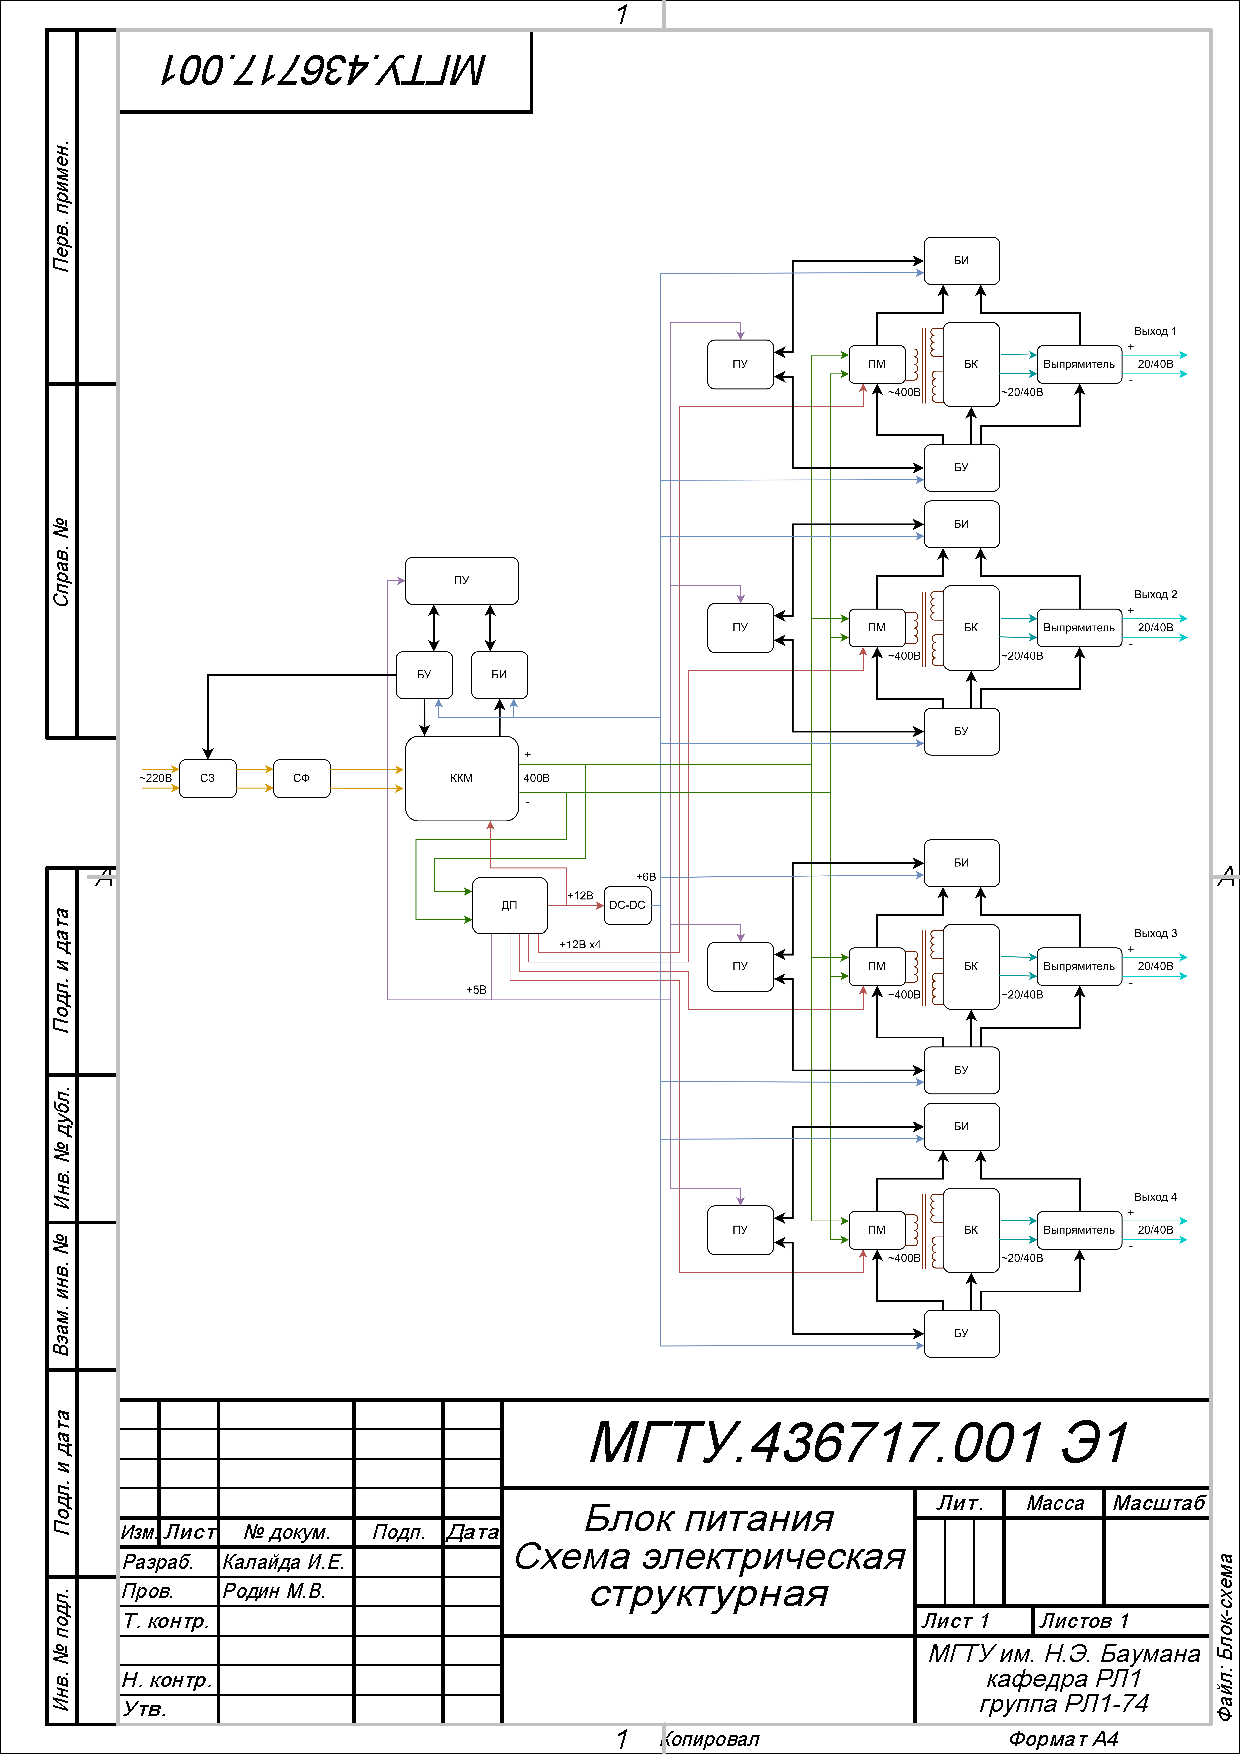
\includepdf[pages=-,fitpaper]{Чертежи/Блок-схема.pdf}
	
	\pagebreak
	
	\section{Структурная схема лабораторного блока питания}\label{app:functional_schem}
	\pagebreak
	
	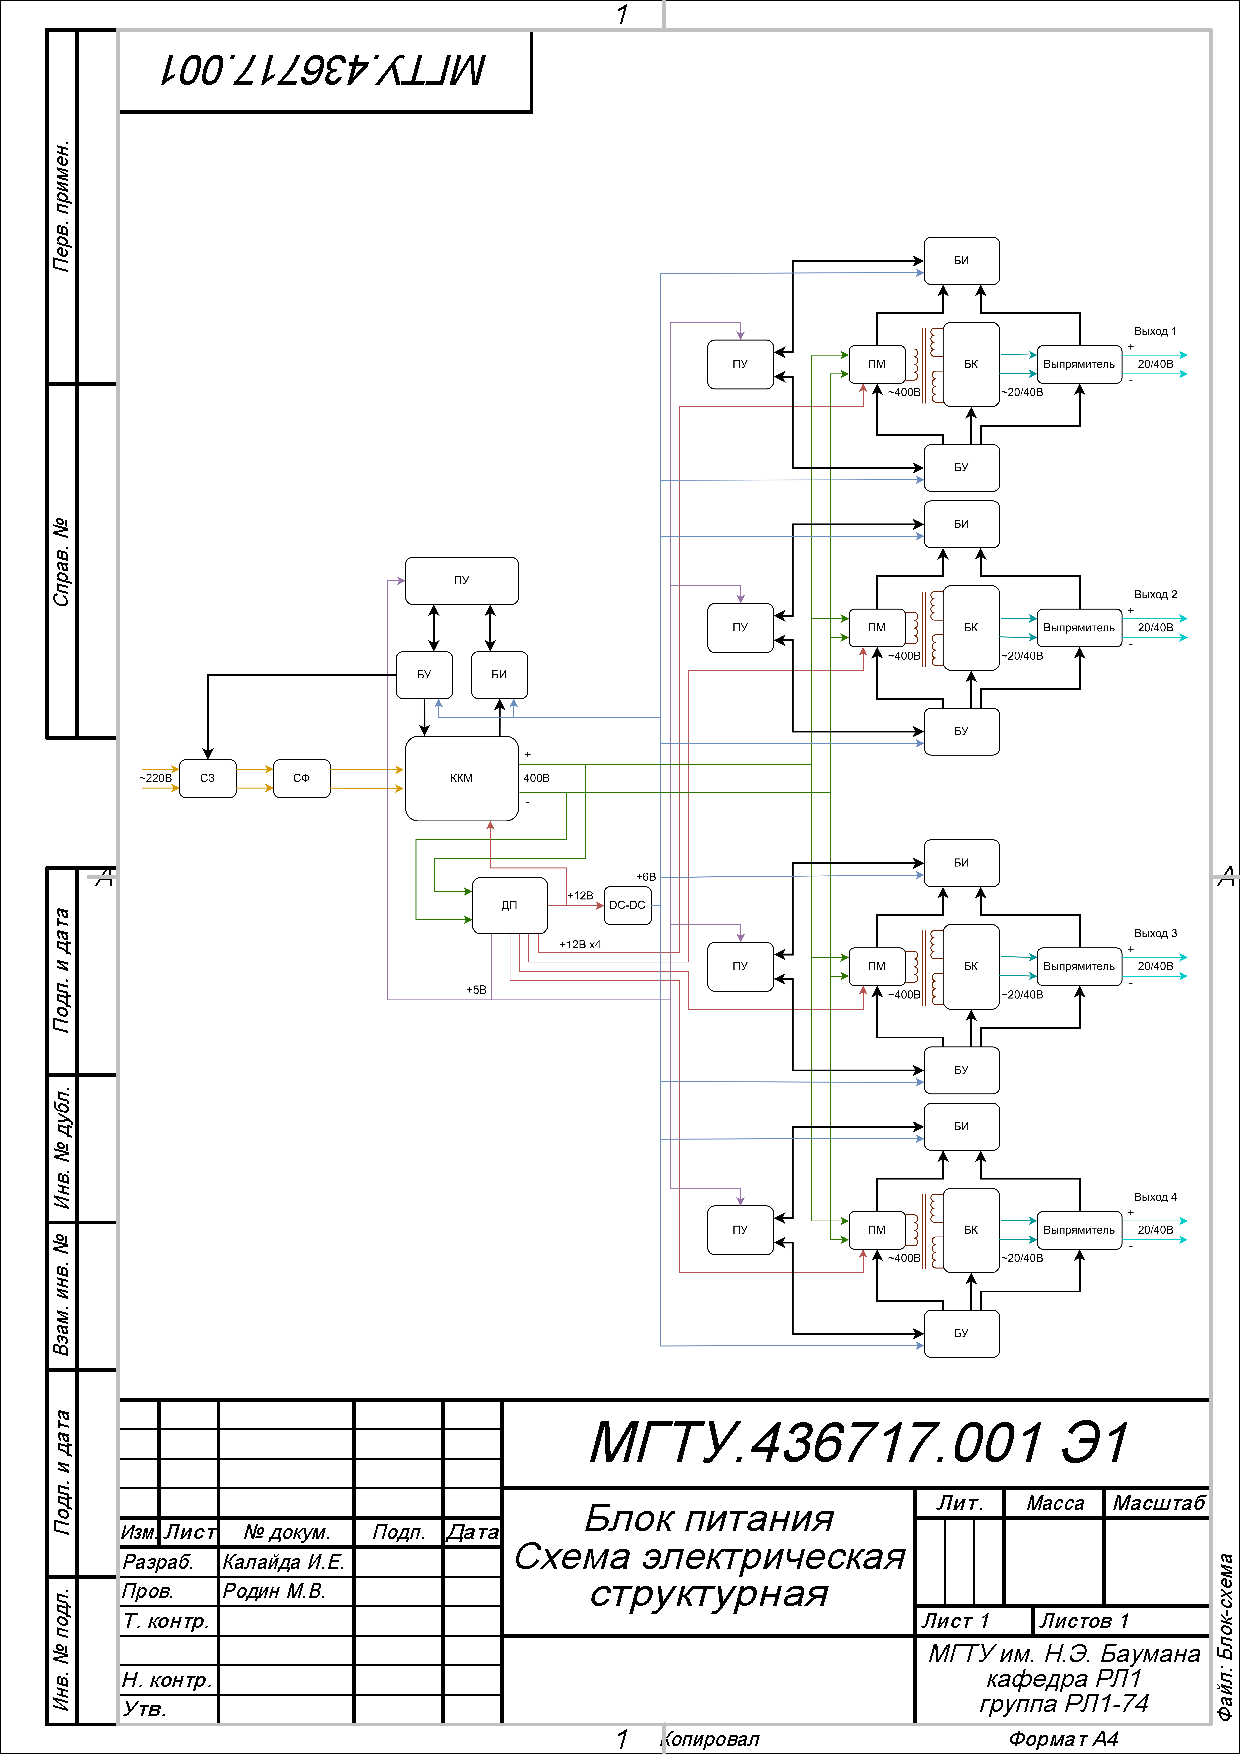
\includepdf[pages=-,fitpaper]{Чертежи/Блок-схема.pdf}
	
	\pagebreak
	
	\section{Принципиальная схема блока дежурного питания}\label{app:support_schem}
	\pagebreak
	
	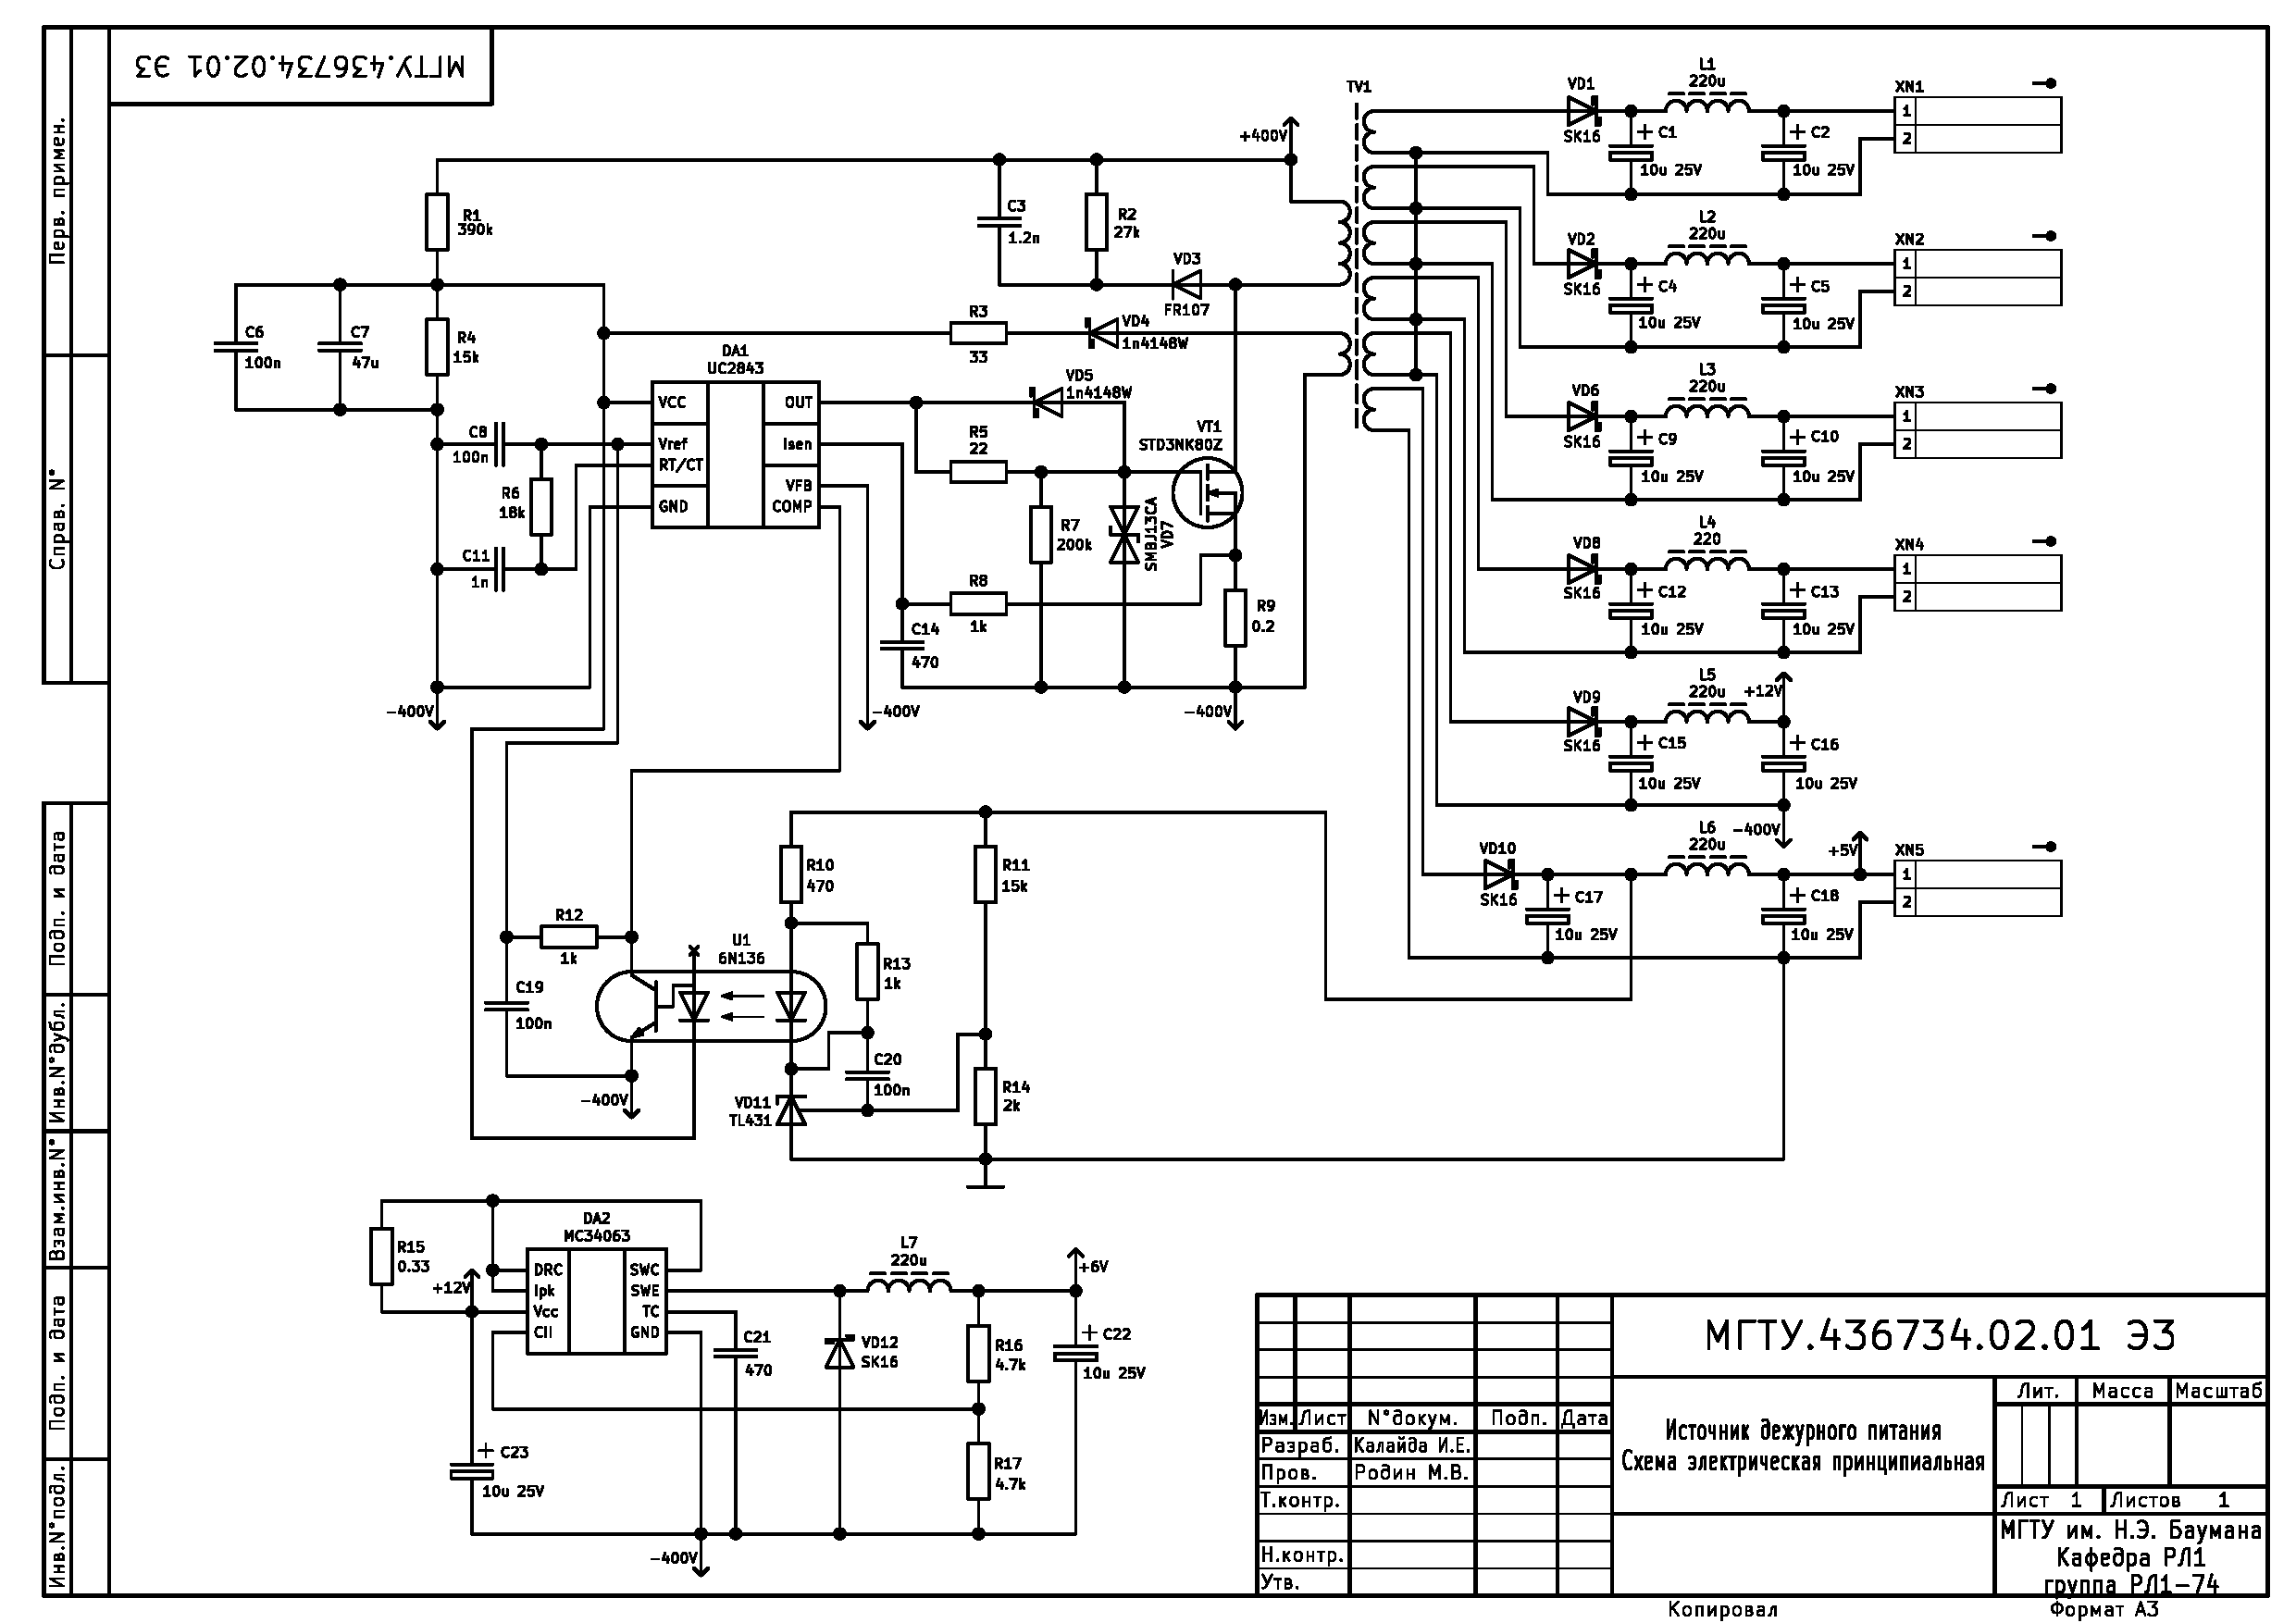
\includepdf[pages=-,fitpaper]{Чертежи/DP-Schem.pdf}
	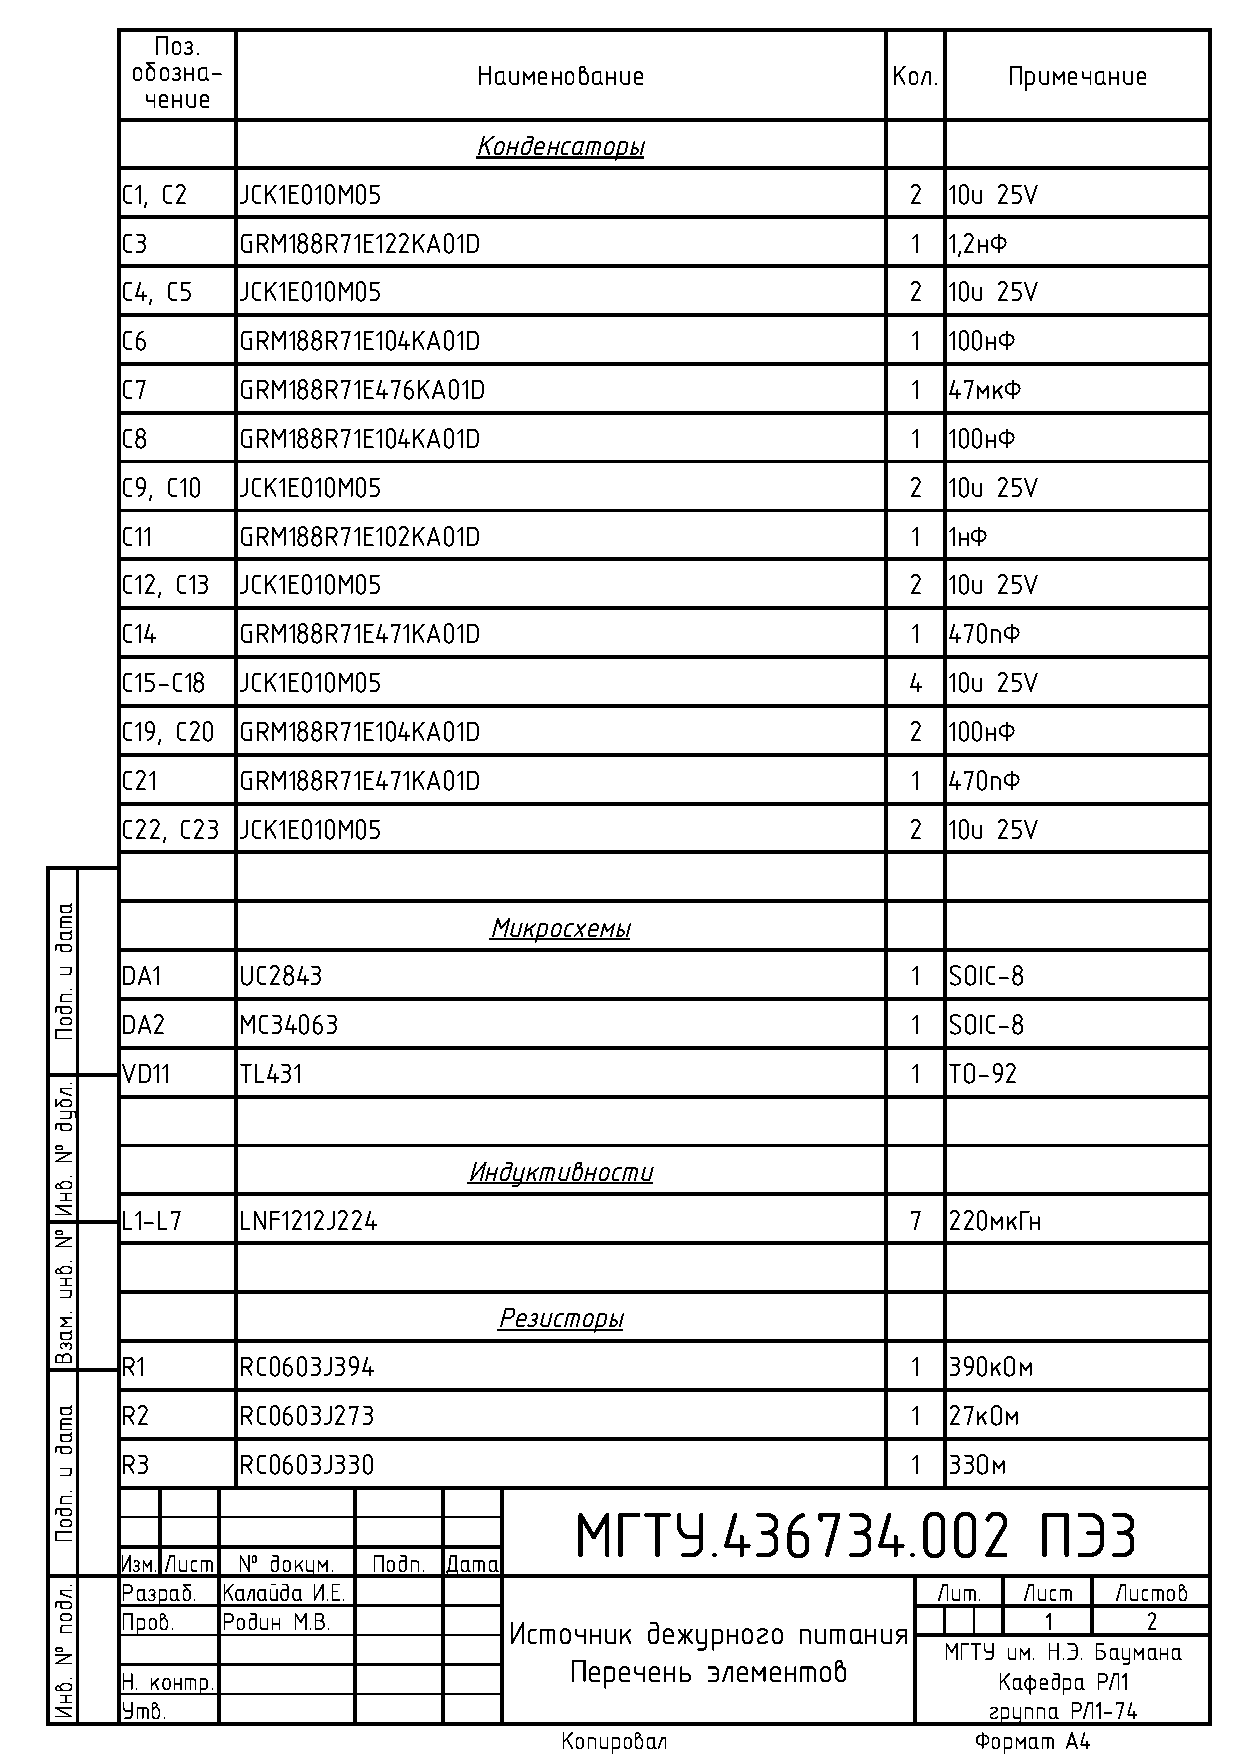
\includepdf[pages=-,fitpaper]{Чертежи/Перечень.pdf}
	
	\pagebreak
	
	\section{Чертежи корпуса 19'}\label{app:solid-19}
	\pagebreak

	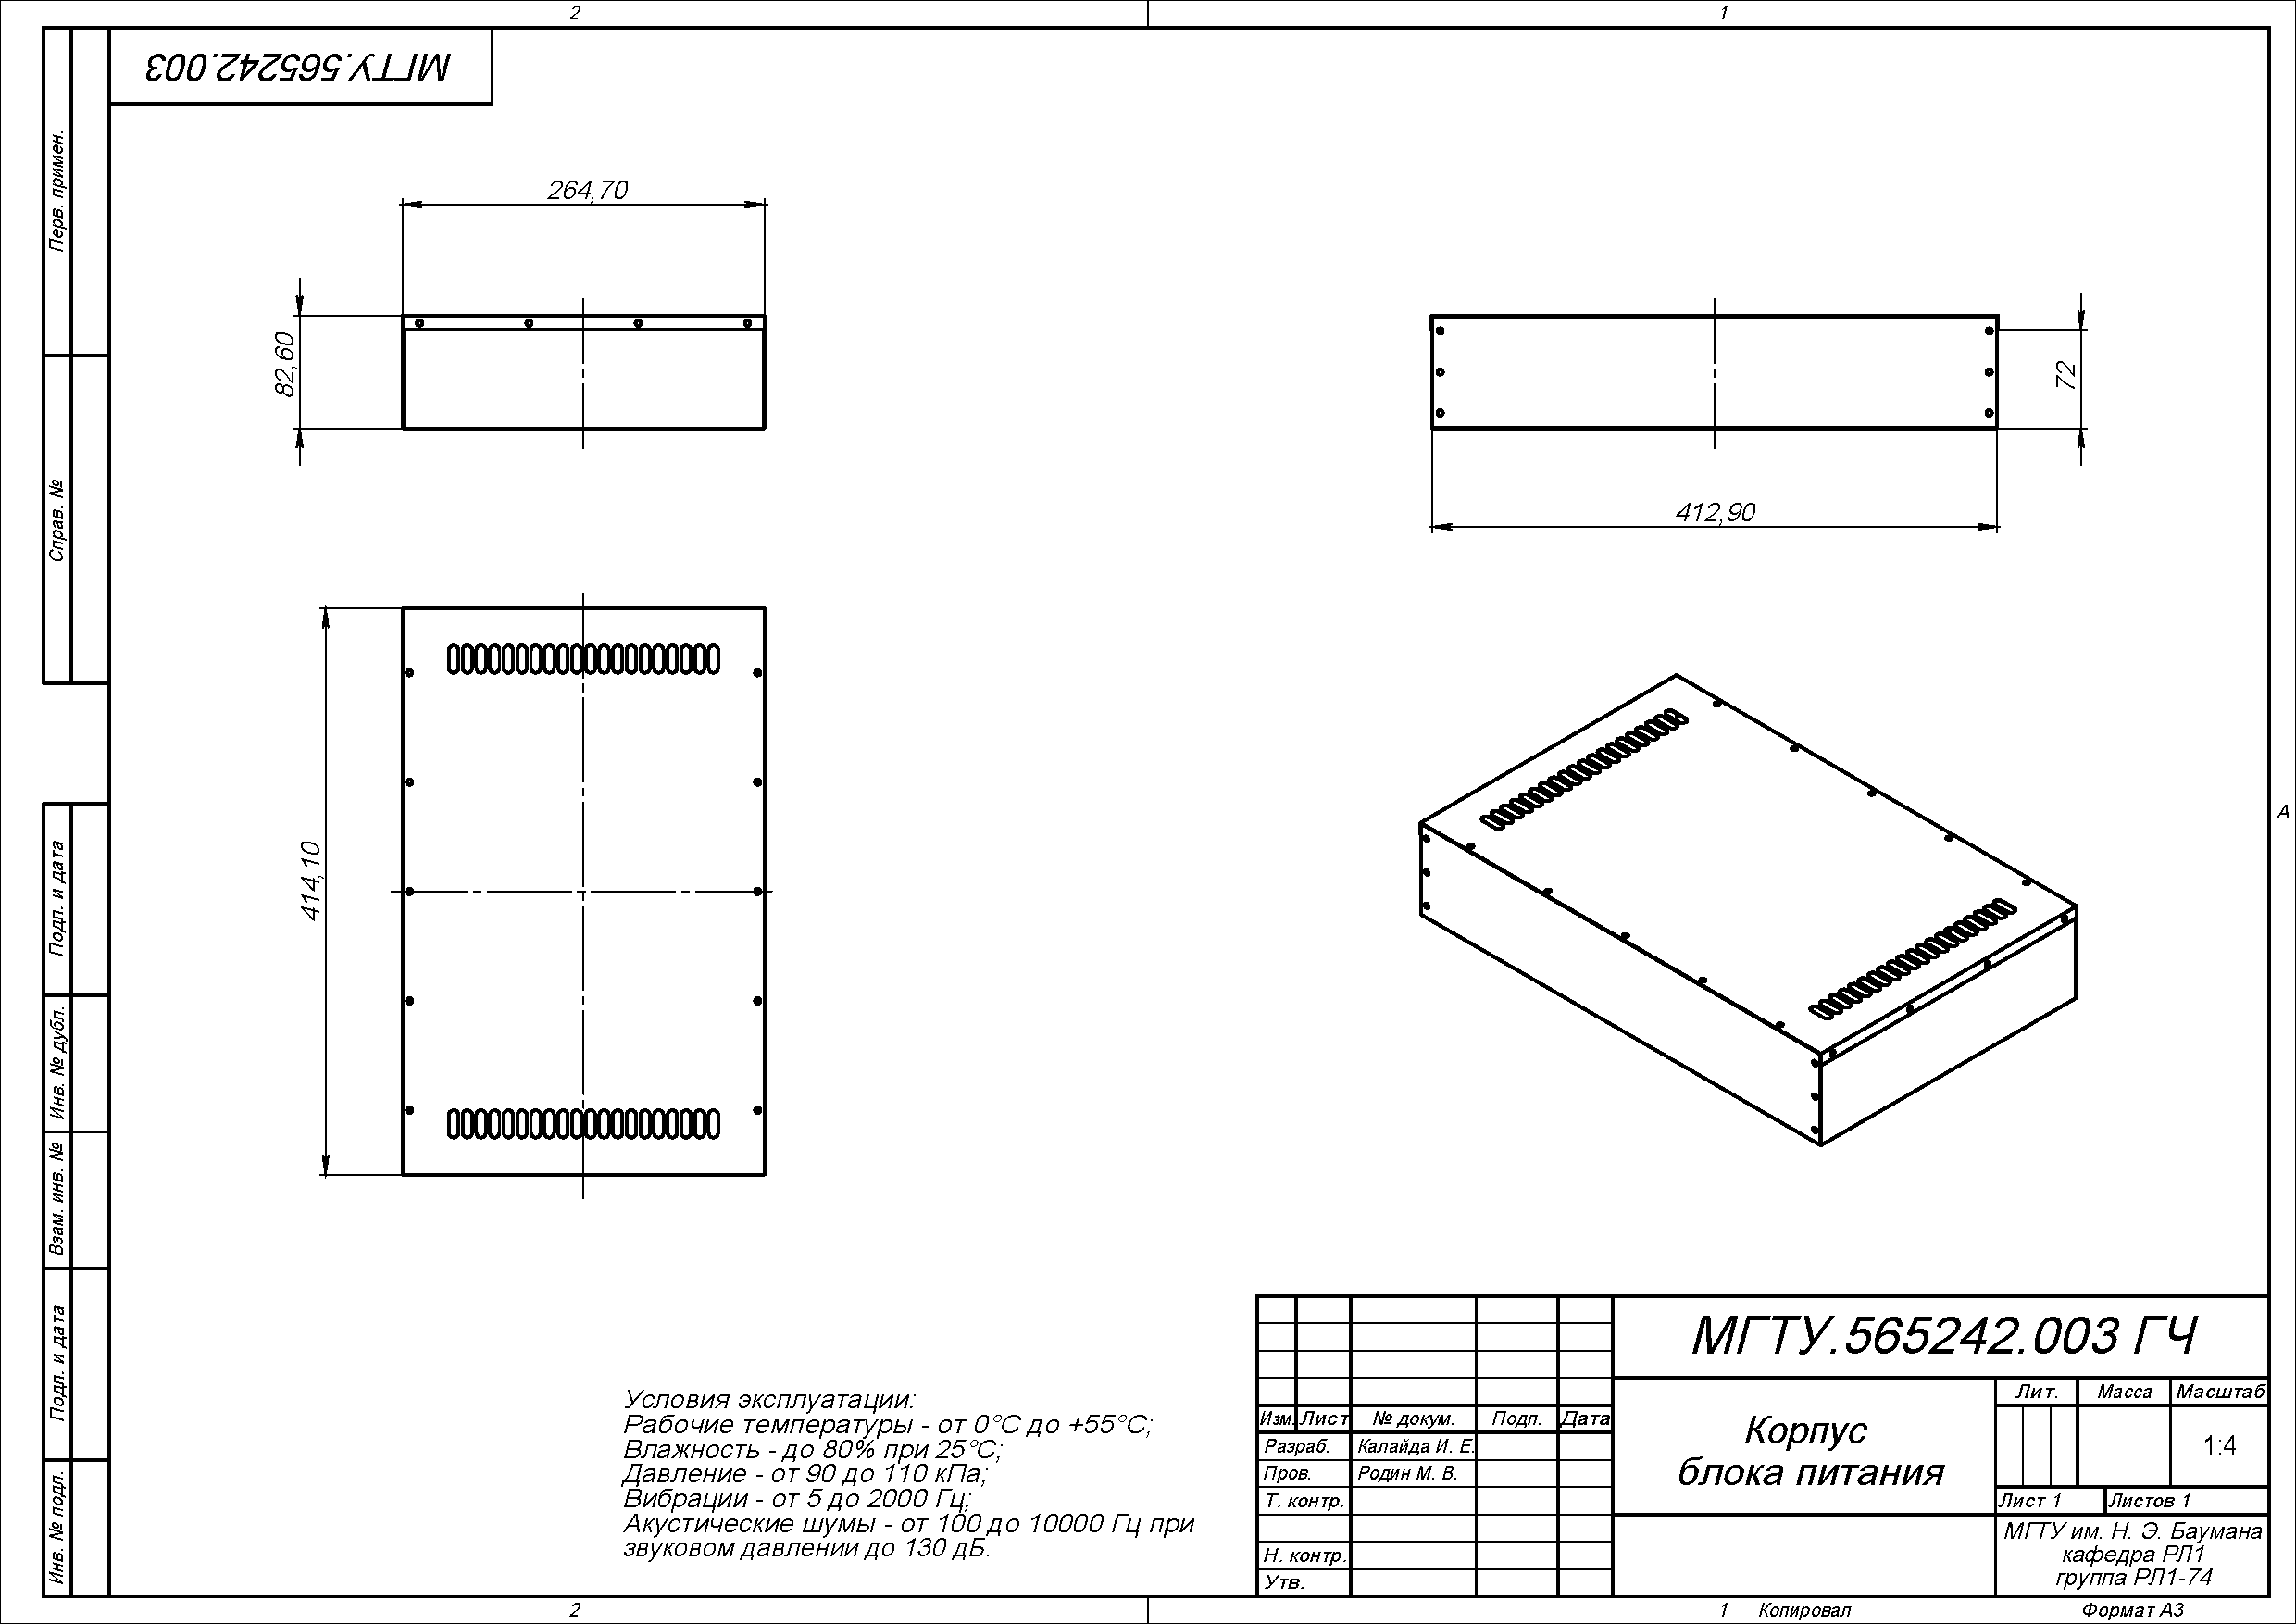
\includepdf[pages=-,fitpaper]{Чертежи/Rack19ich2U.pdf}
	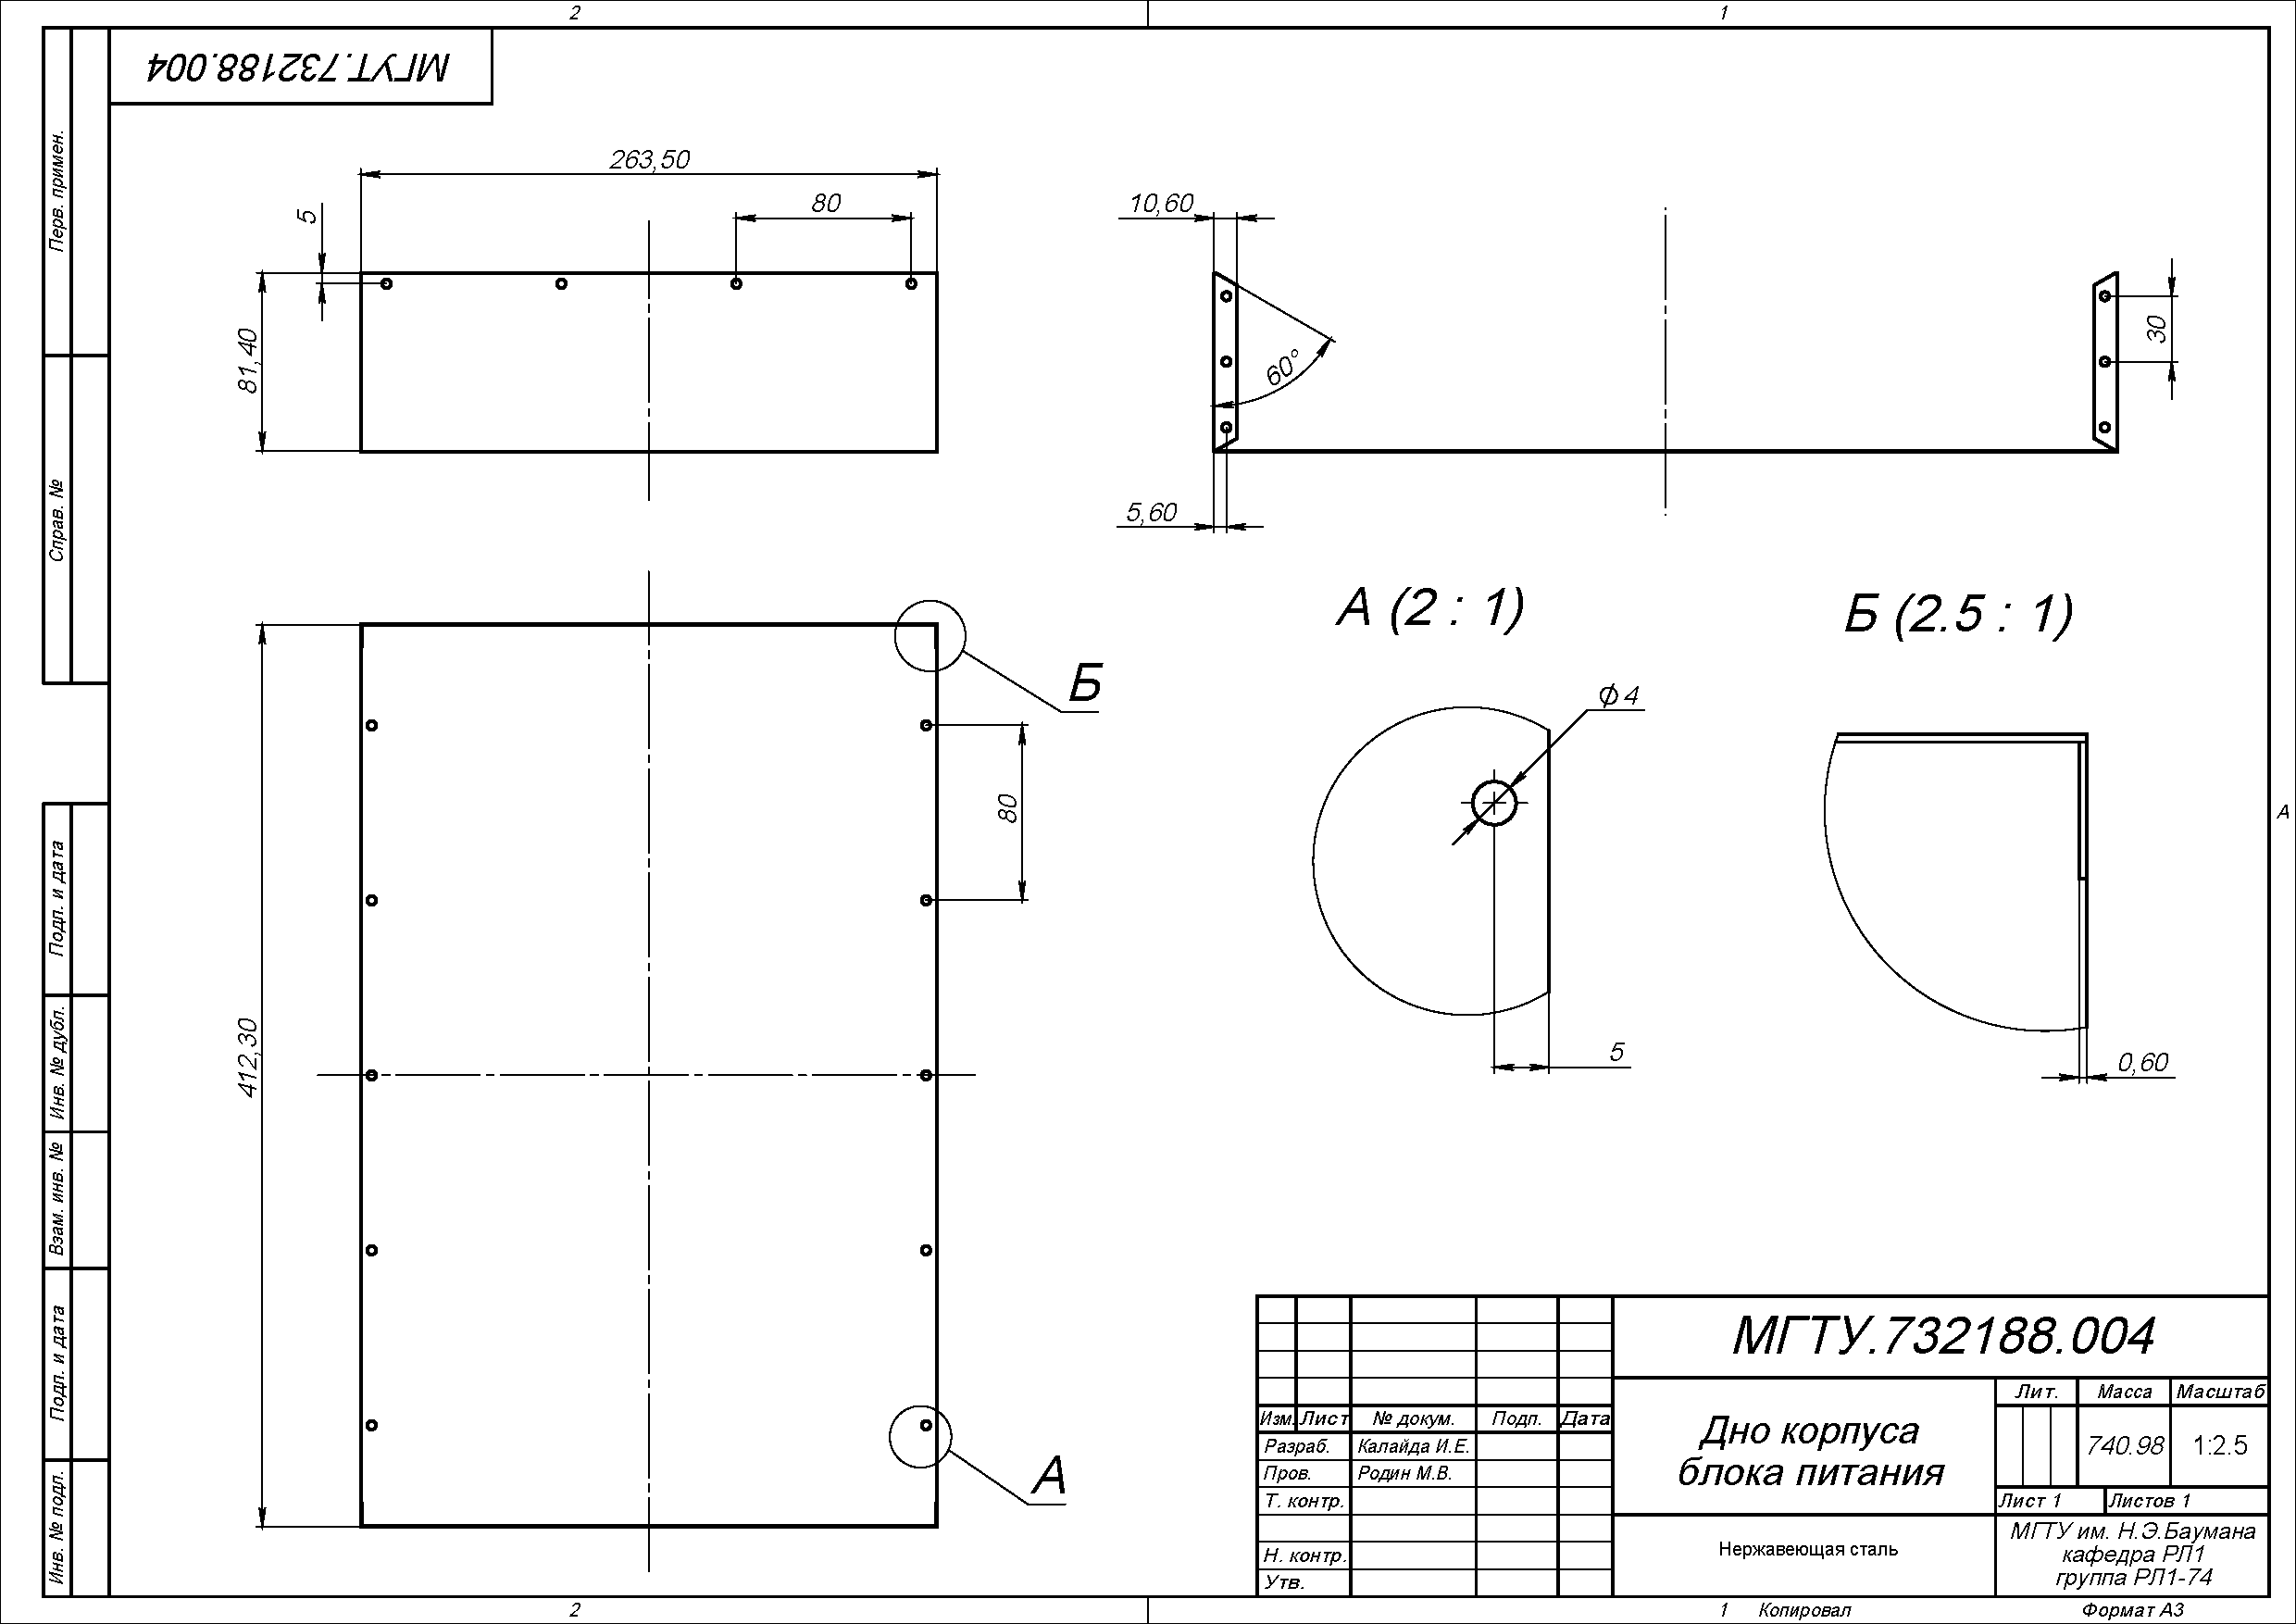
\includepdf[pages=-,fitpaper]{Чертежи/RACK19ich2UBottom.pdf}
	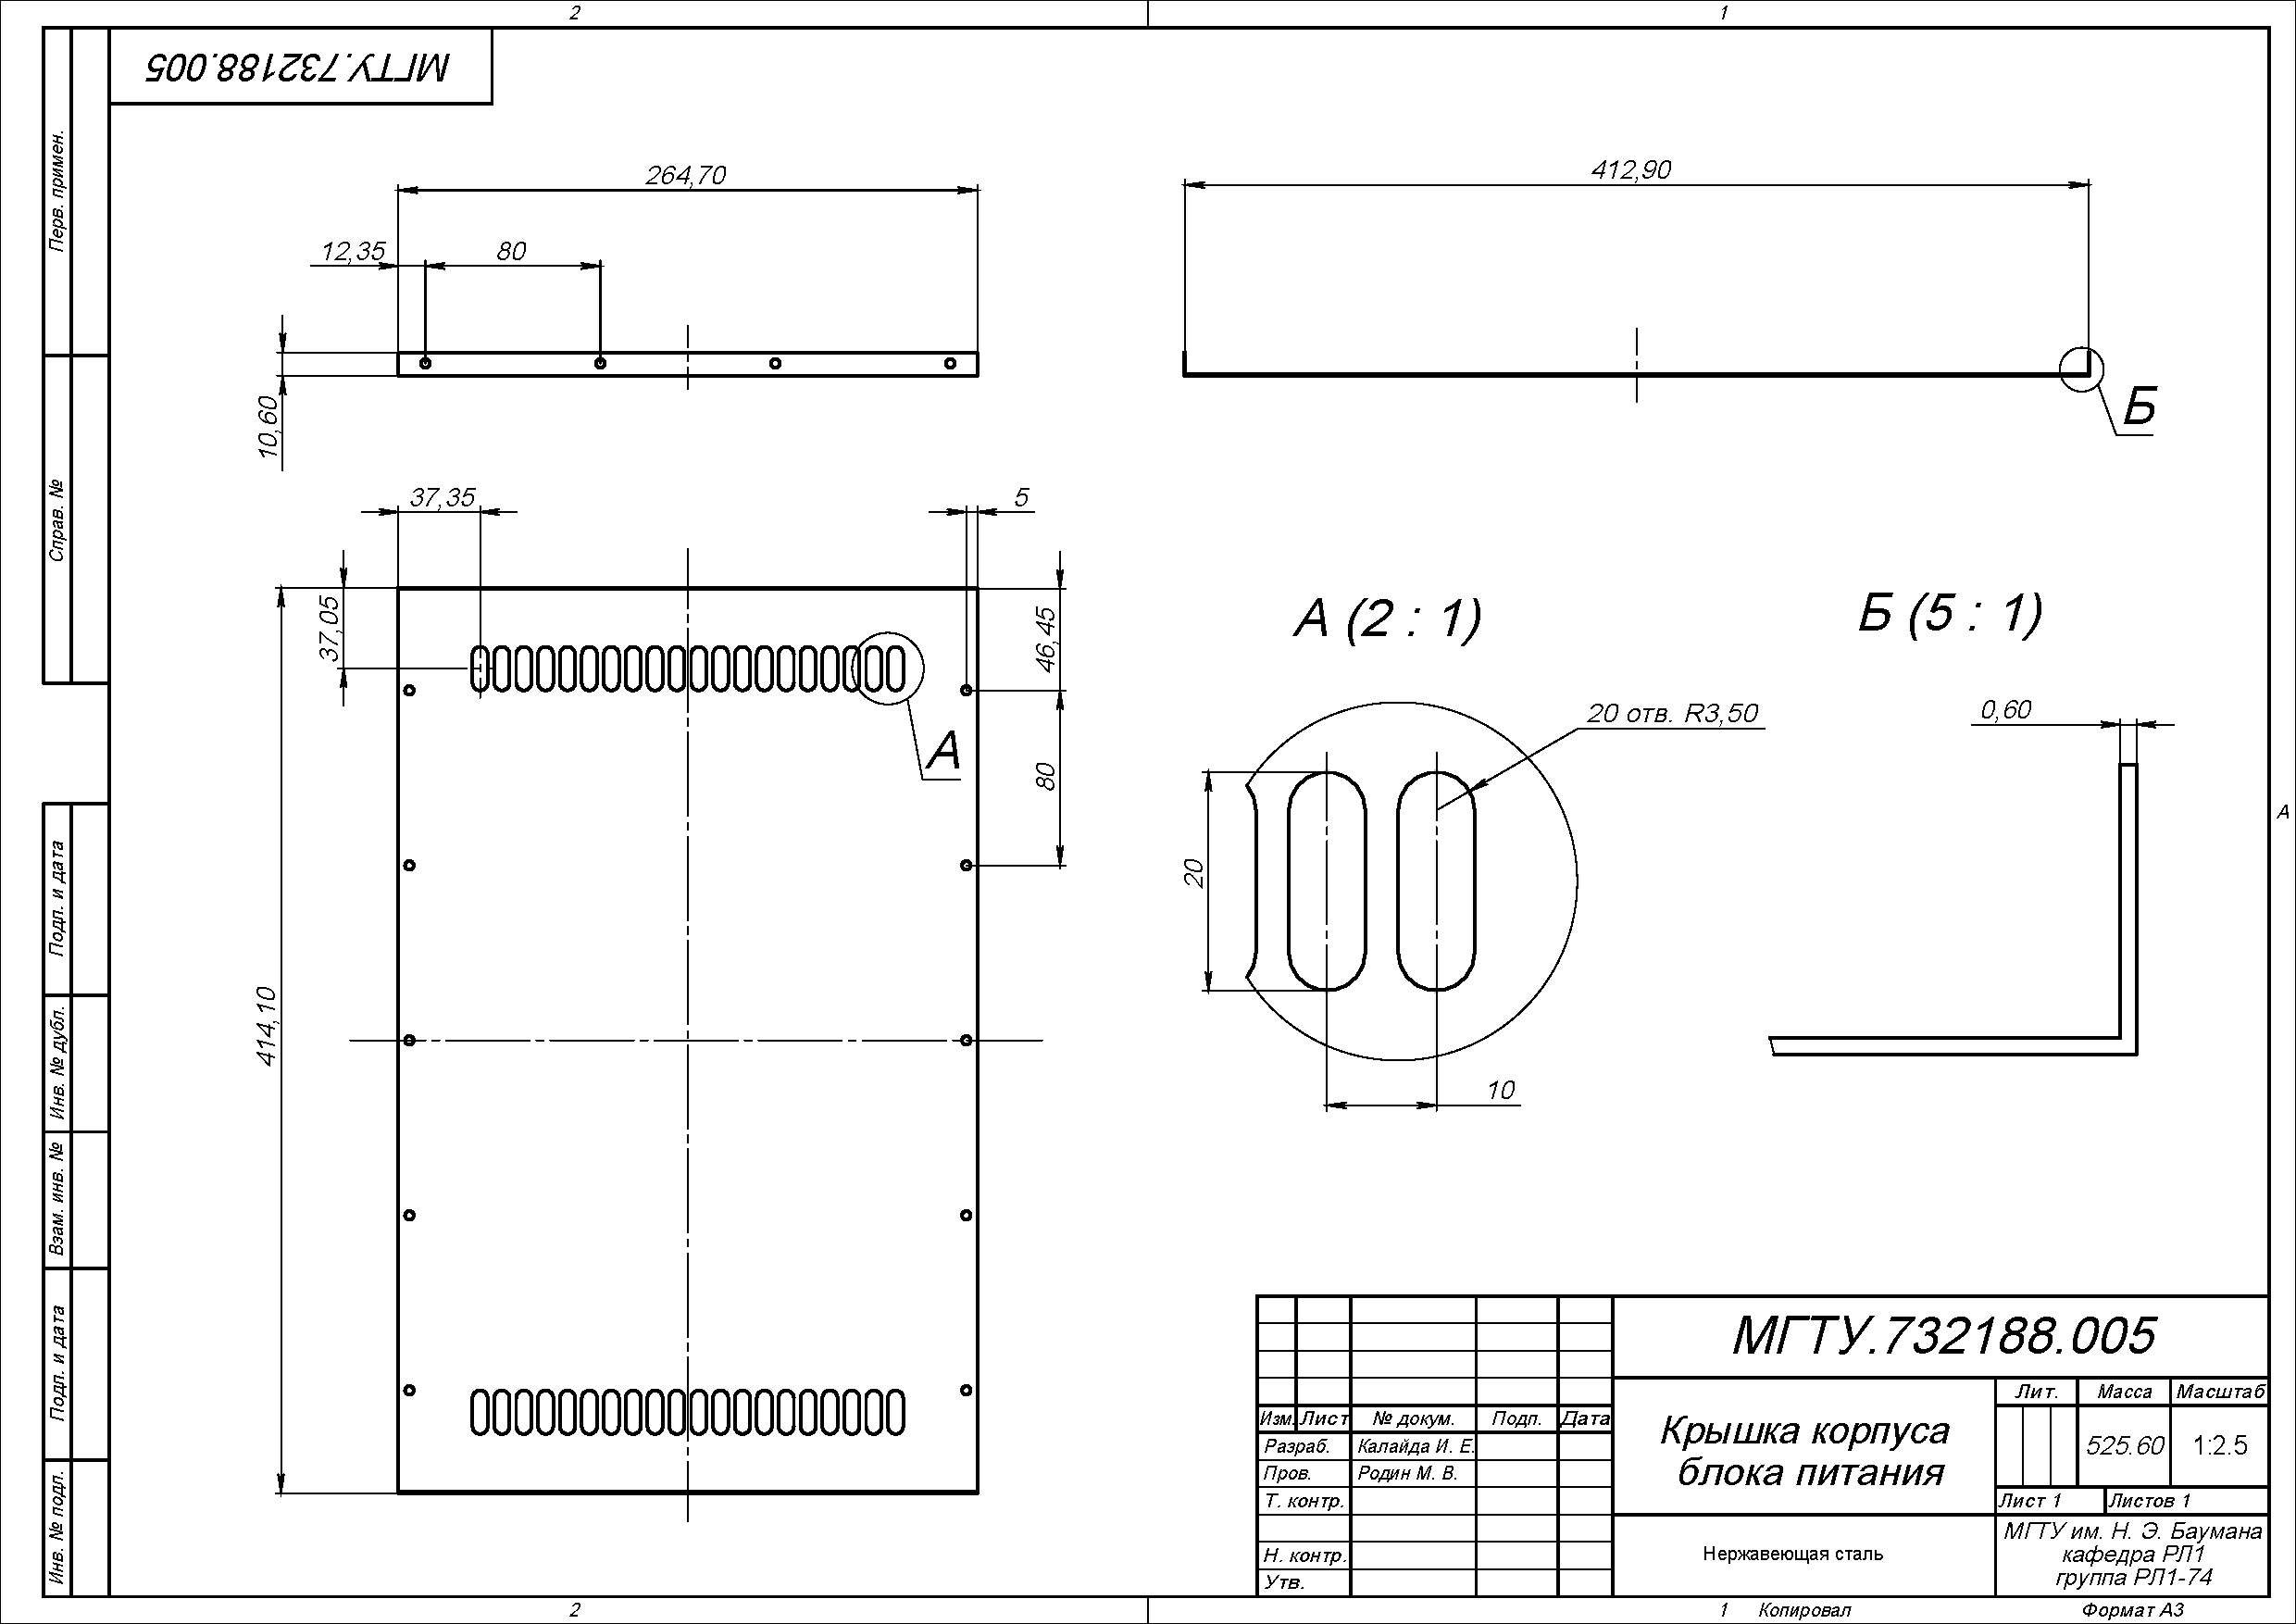
\includepdf[pages=-,fitpaper]{Чертежи/RACK19ich2UTop.pdf}
	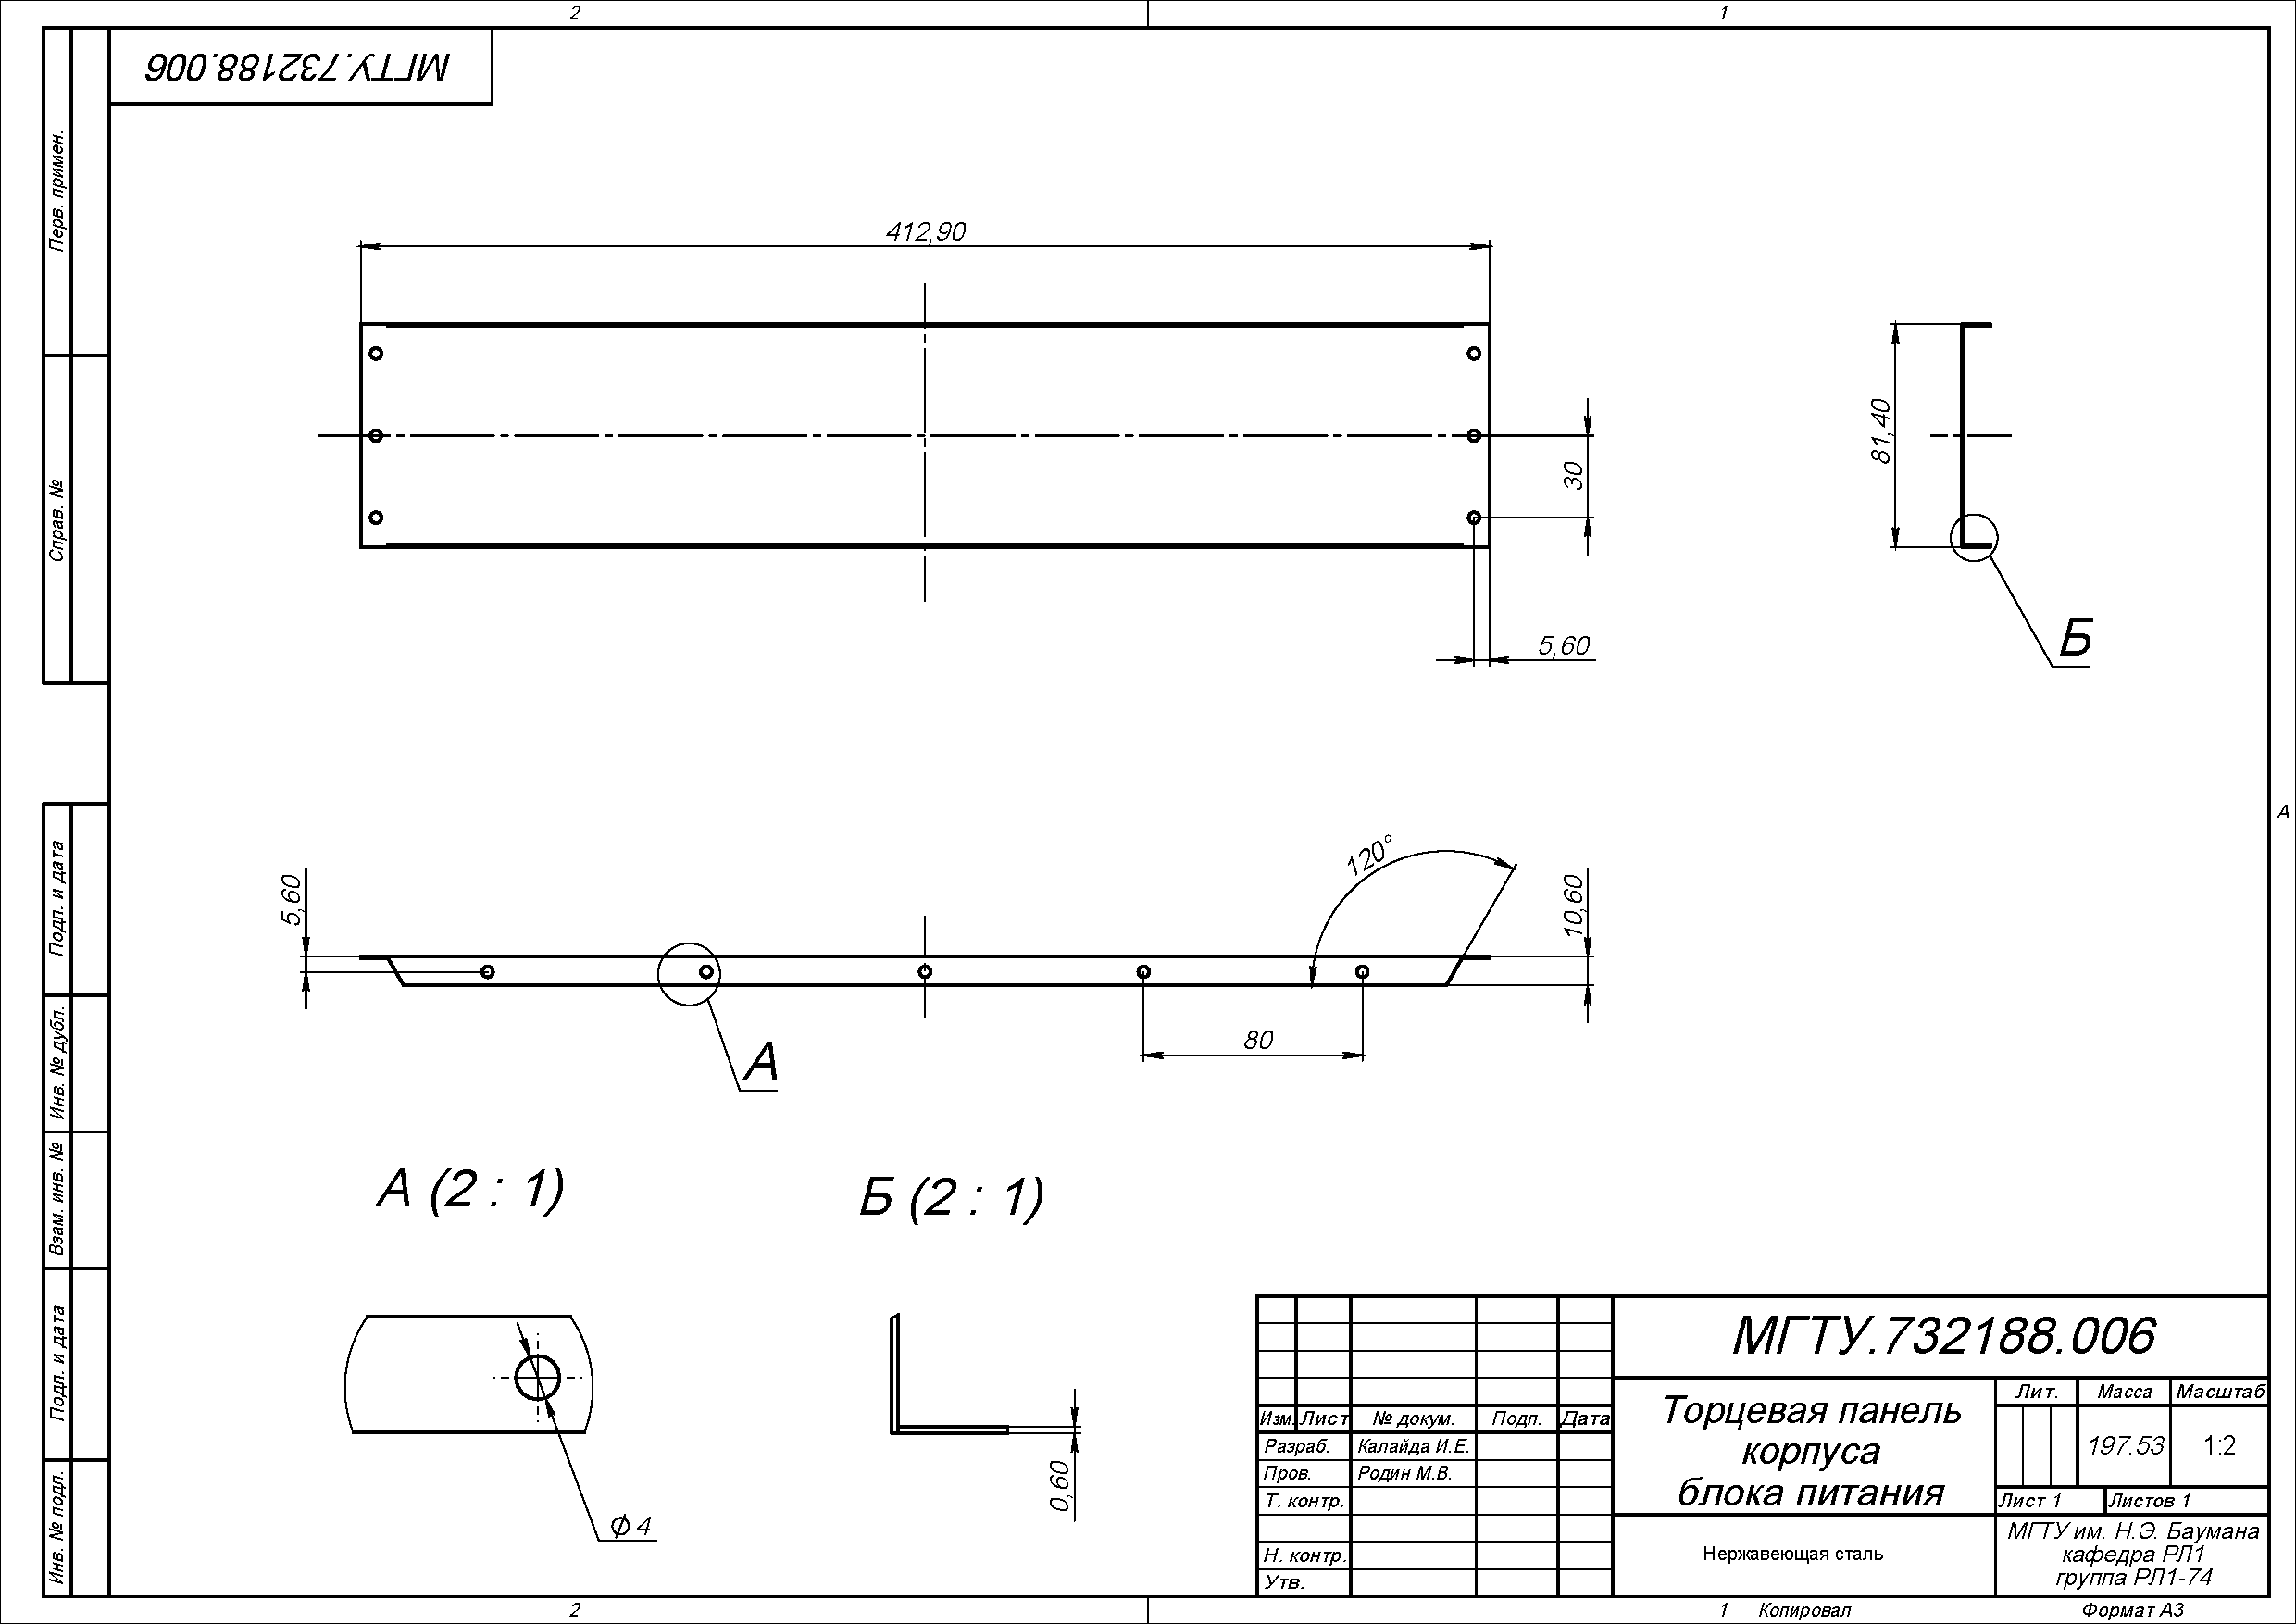
\includepdf[pages=-,fitpaper]{Чертежи/RACK19ich2UFront.pdf}
	
	\pagebreak
	

\end{document}